% \PassOptionsToPackage{quiet}{fontspec}
\documentclass[12pt,a4paper,UTF8]{article}
\usepackage{thesis} % 格式控制
\usepackage{indentfirst} 
\setlength{\parindent}{2em} % 控制首行缩进   
\addtolength{\parskip}{3pt} % 控制段落距离  
\onehalfspacing % 1.5倍行距  
\graphicspath{{../assets/}} % 指定图片所在文件夹  


\usepackage{dirtree}
\classname{智能控制技术}  % 设置课程名称
\expname{永磁同步电机调速}
\makepagestyle{\printexpname}{\printclassname ~实验报告}

\begin{document}
\maketitlepage{\printexpname}{教7 304}{PhilFan}{19260817}{\today}{刘山\ 刘禹骏} %封面页 

\maketoc    %目录页


\section{背景介绍}
电机是新能源汽车的三大核心零部件之一,被誉为新能源汽车的“心脏”。而由于电动汽车的空间限制和使用环境的要求,传统的电力电子与电机技术已经难以满足其高性能、小尺寸和严格的环境温度要求。因此永磁电机作为电动汽车电机驱动系统的关键技术之一,受到广泛关注。

近年来,政府出台了多项政策支持国内纯电动汽车及插电式混合动力汽车在内的新能源汽车的发展。如《新能源汽车产业发展规划(2021-2035)》中,十分明确提出2025年我国新能源汽车新车销售量达到汽车新车销售总量的20\%左右。规划的出台极大地鼓舞了自主品牌汽车新能源产业的上下游,产业呈现爆发式增长势头。

永磁同步电机(PMSM)是一种在转子上采用永磁体作为励磁源的同步电机。相比传统同步电机,PMSM具有结构简单、效率高、功率密度大、调速性能好等优点,在伺服驱动、电动汽车等领域有广泛应用\cite{zhihu2}。


在秋冬学期,我学习了另一门《运动控制》的课程。课上老师提到了有关电机调速的问题我比较感兴趣,所以本次大作业我选择了永磁同步电机调速作为研究对象。(另外在运动控制的大作业中,我做的是PID倒立摆平衡小车,把智能控制中学到的专家控制和模糊控制算法做了应用,感觉还是很有意思的)


\subsection{永磁同步电机数学模型}
永磁同步电机的数学模型可以通过以下方程描述\cite{DGJS202306019}:


\paragraph{d轴电流方程}
\begin{equation}
\frac{dI_d}{dt} = \frac{1}{L_d}(V_d - R_sI_d + \omega L_qI_q)
\end{equation}
其中:
\begin{itemize}
\item $I_d$ 是d轴电流
\item $V_d$ 是d轴电压
\item $R_s$ 是定子电阻
\item $\omega$ 是角速度
\item $L_q$ 和 $L_d$ 分别是q轴和d轴的电感
\item $I_q$ 是q轴电流
\end{itemize}

\paragraph{q轴电流方程}
\begin{equation}
\frac{dI_q}{dt} = \frac{1}{L_q}(V_q - R_sI_q - \omega L_dI_d - \omega\psi_f)
\end{equation}
其中:
\begin{itemize}
\item $I_q$ 是q轴电流
\item $V_q$ 是q轴电压
\item $\psi_f$ 是永磁体磁链
\end{itemize}

\paragraph{转速方程}
\begin{equation}
\frac{d\omega}{dt} = \frac{1}{J}(T_e - T_L - B\omega)
\end{equation}
其中:
\begin{itemize}
\item $\omega$ 是角速度
\item $J$ 是转动惯量
\item $T_e$ 是电磁转矩
\item $T_L$ 是负载转矩
\item $B$ 是阻尼系数
\end{itemize}

\paragraph{电磁转矩方程}
\begin{equation}
T_e = \frac{3}{2}p(\psi_fI_q + (L_d - L_q)I_dI_q)
\end{equation}
其中:
\begin{itemize}
\item $T_e$ 是电磁转矩
\item $p$ 是极对数
\item $\psi_f$ 是永磁体磁链
\item $L_d$ 和 $L_q$ 分别是d轴和q轴的电感
\end{itemize}

\section{问题分析}

根据永磁同步电机的数学模型\cite{DGJS202306019},我们可以将系统的输入、输出和状态变量进行分析。系统的输入变量包括d轴电压$V_d$、q轴电压$V_q$以及负载转矩$T_L$。其中$V_d$和$V_q$是控制器的输出量,可以通过控制器进行调节;而$T_L$是外部负载带来的扰动,在实际应用中往往难以准确测量。系统的输出变量是电机转速$\omega$,这也是我们最终需要控制的目标量。状态变量包括d轴电流$I_d$、q轴电流$I_q$和电机转速$\omega$,这些变量完整地描述了系统在任意时刻的状态。通过建立这些变量之间的关系,我们可以设计相应的控制策略来实现对电机转速的精确控制。


\begin{itemize}
    \item \textbf{输入变量:}
    \begin{enumerate}
        \item $V_d$: d轴电压(控制器输出)
        \item $V_q$: q轴电压(控制器输出)
        \item $T_L$: 负载转矩(扰动)
    \end{enumerate}
    \item \textbf{输出变量:}
    \begin{enumerate}
        \item $\omega$: 电机转速(rad/s)
    \end{enumerate}
    \item \textbf{状态变量:}
    \begin{enumerate}
        \item $I_d$: d轴电流
        \item $I_q$: q轴电流
        \item $\omega$: 电机转速
    \end{enumerate}
\end{itemize}

\textbf{S-function建立}

在本实验中,我使用S-function来建立永磁同步电机的simulink模型。

\begin{itemize}
\item \textbf{输入输出定义:} 
  \begin{itemize}
    \item 输入(u): 包括d轴电压$V_d$、q轴电压$V_q$和负载转矩$T_L$
    \item 输出(y): 电机转速$\omega$
    \item 状态变量(x): d轴电流$I_d$、q轴电流$I_q$和转速$\omega$
  \end{itemize}
\item \textbf{初始化函数(mdlInitializeSizes):} 定义系统的基本参数,包括连续状态数量(3个)、输入数量(3个)和输出数量(1个)
\item \textbf{状态方程(mdlDerivatives):} 实现电机的数学模型,包括d轴电流方程、q轴电流方程和转速方程
\end{itemize}

在使用时需要注意以下几点:
\begin{itemize}
\item 确保输入参数的单位统一性
\item 采样时间设为连续(ts = [0 0])以保证仿真精度
\end{itemize}


\begin{lstlisting}[language=Matlab,caption=S-function建立]
    function [sys, x0, str, ts, simStateCompliance] = motor(t, x, u, flag, R_s, L_d, L_q, psi_f, p, J, B)
    switch flag
        case 0
            [sys, x0, str, ts, simStateCompliance] = mdlInitializeSizes();
        case 1
            sys = mdlDerivatives(t, x, u, R_s, L_d, L_q, psi_f, p, J, B);
        case 2
            sys = mdlUpdate(t, x, u);
        case 3
            sys = mdlOutputs(t, x, u);
        case 9
            sys = mdlTerminate(t, x, u);
        otherwise
            DAStudio.error('Simulink:blocks:unhandledFlag', num2str(flag));
    end
end

% 初始化函数
function [sys, x0, str, ts, simStateCompliance] = mdlInitializeSizes()
    % 定义状态、输入、输出的大小
    sizes = simsizes;

    sizes.NumContStates  = 3;  % 连续状态:I_d, I_q, omega
    sizes.NumDiscStates  = 0;  % 无离散状态
    sizes.NumOutputs     = 1;  % 输出:omega
    sizes.NumInputs      = 3;  % 输入:V_d, V_q, T_L
    sizes.DirFeedthrough = 0;  % 无直接传递
    sizes.NumSampleTimes = 1;  % 一个采样时间

    sys = simsizes(sizes);

    x0 = [0; 0; 0]; % 初始状态:I_d, I_q, omega
    str = [];
    ts = [0 0]; % 连续时间系统
    simStateCompliance = 'UnknownSimState'; % 状态兼容性
end

% 更新函数(此处为空,因为是连续系统)
function sys = mdlUpdate(~, ~, ~)
    sys = [];
end

% 输出函数
function sys = mdlOutputs(~, x, ~)
    sys = [x(3)];
end

% 终止函数
function sys = mdlTerminate(~, ~, ~)
    % 终止时执行清理操作(如果需要)
    sys = [];
end

% 动态方程求解
function sys = mdlDerivatives(~, x, u, R_s, L_d, L_q, psi_f, p, J, B)
    % 参数定义
    % R_s = 0.01;     % 定子电阻
    % L_d = 0.001;    % d 轴电感
    % L_q = 0.0015;   % q 轴电感
    % psi_f = 0.1;    % 永磁体磁链
    % p = 4;          % 极对数
    % J = 0.01;       % 转动惯量
    % B = 0.001;      % 阻尼系数

    % 输入提取
    V_d = u(1); % d 轴电压
    V_q = u(2); % q 轴电压
    T_L = u(3); % 负载转矩

    % 状态提取
    I_d = x(1); % d 轴电流
    I_q = x(2); % q 轴电流
    omega = x(3); % 转速

    % 电磁转矩计算
    T_e = (3/2) * p * (psi_f * I_q + (L_d - L_q) * I_d * I_q);

    % d 轴电流微分方程
    dId_dt = (1 / L_d) * (V_d - R_s * I_d + omega * L_q * I_q);

    % q 轴电流微分方程
    dIq_dt = (1 / L_q) * (V_q - R_s * I_q - omega * L_d * I_d - omega * psi_f);

    % 转速微分方程
    domega_dt = (1 / J) * (T_e - T_L - B * omega);

    % 返回微分方程结果
    sys = [dId_dt; dIq_dt; domega_dt];
end
\end{lstlisting}

建立好的电机模型在simulink中如下图所示


\begin{figure}[htbp] \centering 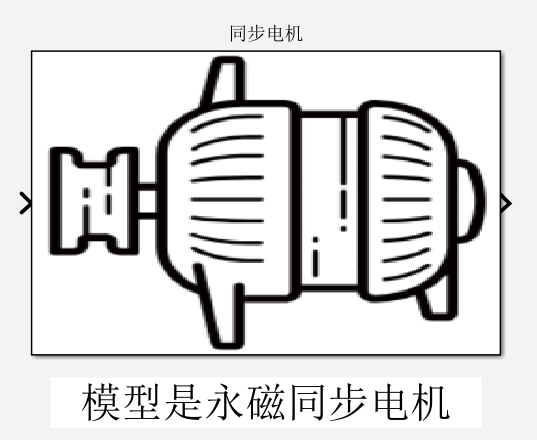
\includegraphics[width=0.4\textwidth]{2024-12-30-11-32-16.png} \caption{建立的电机模型}\end{figure}

这里我使用了S-function的模型封装MASK功能,将参数设置为常数使用输入框给定,这样就可以让我便于调整参数,进行修改。


\begin{figure}[!htbp]
    \centering
    \begin{minipage}[b]{0.45\linewidth}
        \centering
        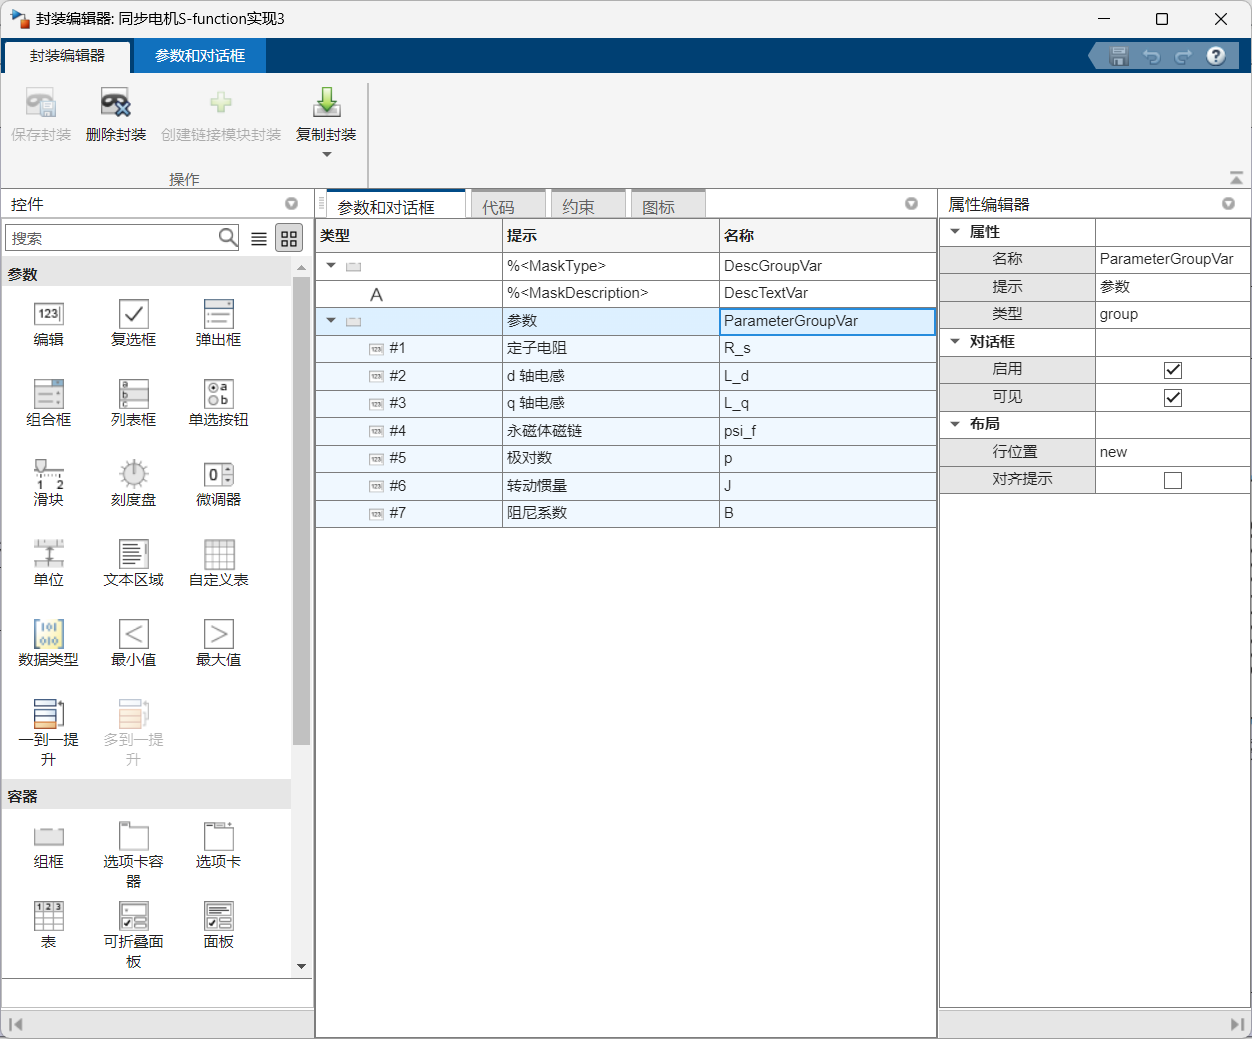
\includegraphics[width=0.7\textwidth]{2024-12-30-11-45-42.png} \caption{S-function模型封装}
         
    \end{minipage}%
    \begin{minipage}[b]{0.45\linewidth}
        \centering
        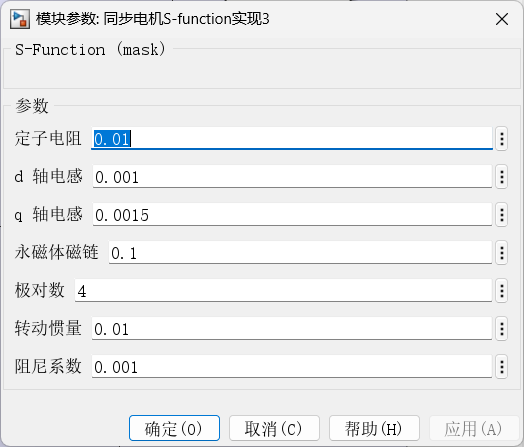
\includegraphics[width=0.7\textwidth]{2024-12-30-11-45-08.png} \caption{S-function模型封装MASK}
    \end{minipage}
\end{figure}

\clearpage
\section{PID建模控制}
\subsection{PID控制器设计}
PID控制器是一种经典的反馈控制器,由比例(P)、积分(I)和微分(D)三部分组成。对于永磁同步电机的速度控制,PID控制器的输出可以表示为:

\begin{equation}
u(t) = K_p e(t) + K_i \int_0^t e(\tau)d\tau + K_d \frac{de(t)}{dt}
\end{equation}

其中:
\begin{itemize}
\item $u(t)$ 是控制器输出
\item $e(t)$ 是误差信号,即参考速度与实际速度之差
\item $K_p$ 是比例增益
\item $K_i$ 是积分增益  
\item $K_d$ 是微分增益
\end{itemize}

使用simulink中的PID模块,我们把电机模型和PID控制器连接起来,如下图所示

\begin{figure}[htbp] \centering 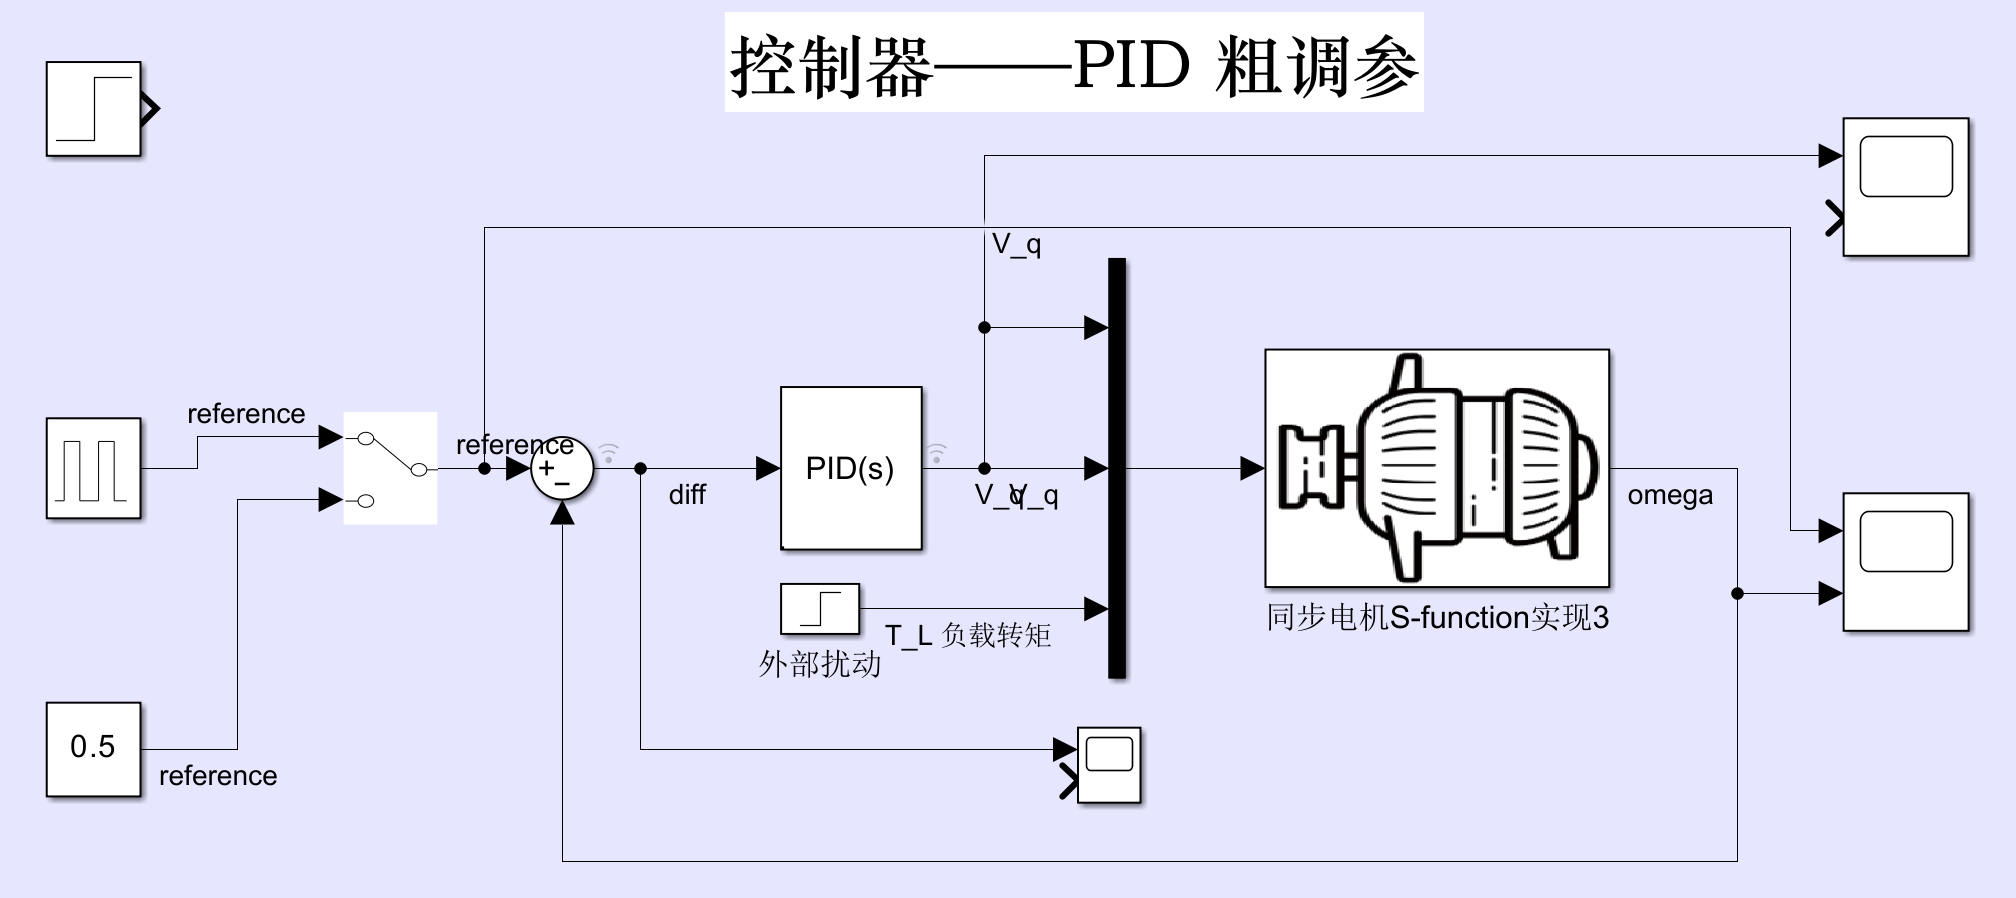
\includegraphics[width=0.7\textwidth]{2024-12-30-11-38-41.png} \caption{PID控制模型}\end{figure}


\subsection{PID调参}


在PID控制器的调参过程中,我采用了以下步骤:

\begin{enumerate}
    \item 首先调整比例参数$K_p$
    \begin{itemize}
        \item 将$K_i$和$K_d$设为0,仅使用P控制
        \item 从小到大逐步增加$K_p$,直到系统响应速度合适
        \item 此时系统会存在稳态误差,但响应较快
    \end{itemize}

    \item 调整积分参数$K_i$
    \begin{itemize}
        \item 在合适的$K_p$基础上,逐步增加$K_i$
        \item $K_i$的作用是消除稳态误差
        \item $K_i$太大会导致超调和震荡,太小则收敛太慢
        \item 通过反复测试找到合适的$K_i$值,使系统既能消除稳态误差,又不会产生过大的超调
    \end{itemize}

    \item 最后微调微分参数$K_d$
    \begin{itemize}
        \item $K_d$的作用是抑制超调和震荡
        \item $K_d$值不宜过大,否则会引入高频噪声,使系统不稳定
    \end{itemize}
\end{enumerate}

通过以上调参过程,最终得到了一组PID参数,系统能够快速跟踪阶跃和方波信号。

\begin{figure}[htbp] \centering 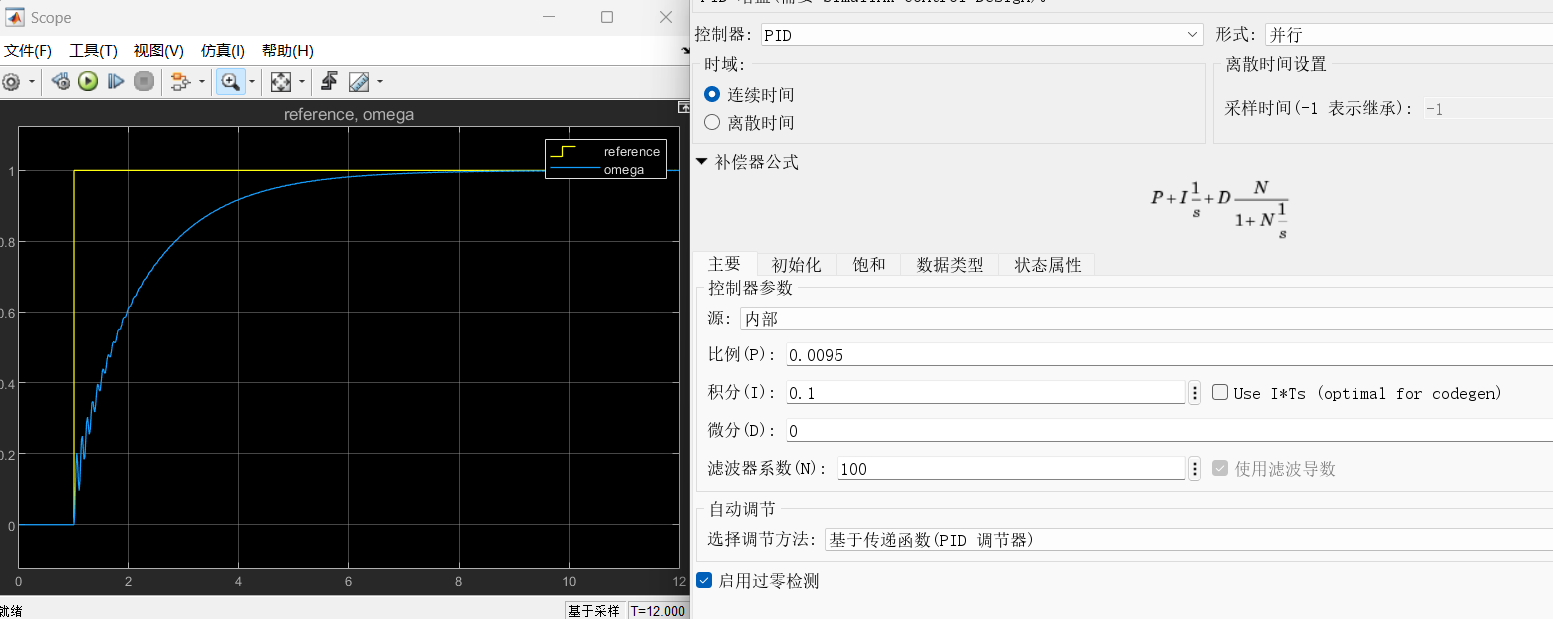
\includegraphics[width=0.7\textwidth]{2024-12-30-11-52-55.png} \caption{跟踪阶跃信号}\end{figure}

图\ref{fig:pid_tuning_result}是PID调参结果,从左到右依次是响应与给定信号,误差,输出电压


\begin{figure}[htbp] \centering 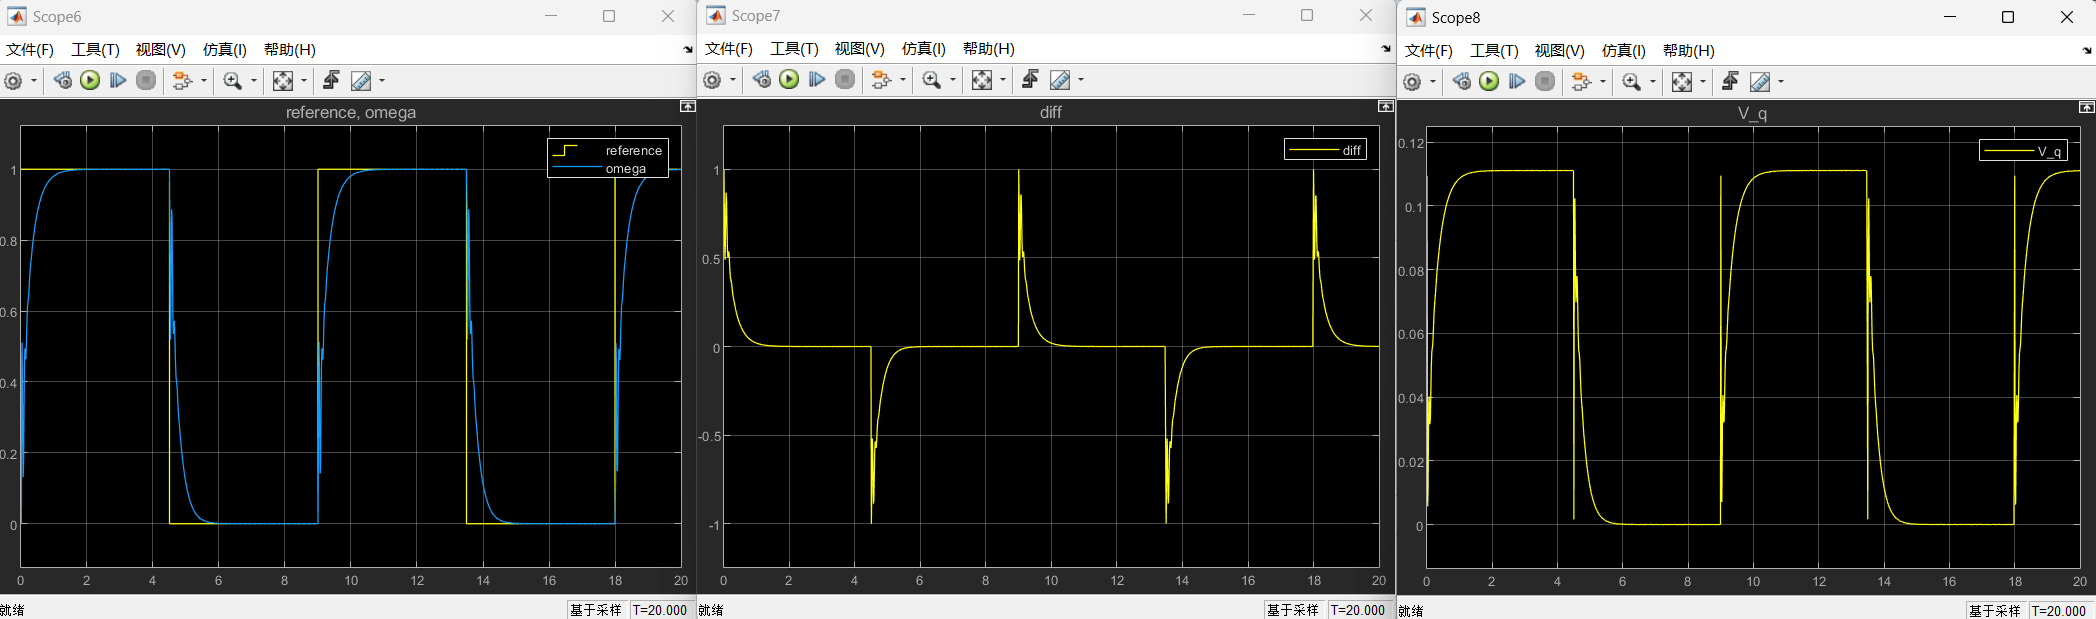
\includegraphics[width=\textwidth]{2024-12-30-11-48-55.png} \caption{PID调参结果,跟踪方波信号} \label{fig:pid_tuning_result}\end{figure}

\begin{figure}[htbp] \centering 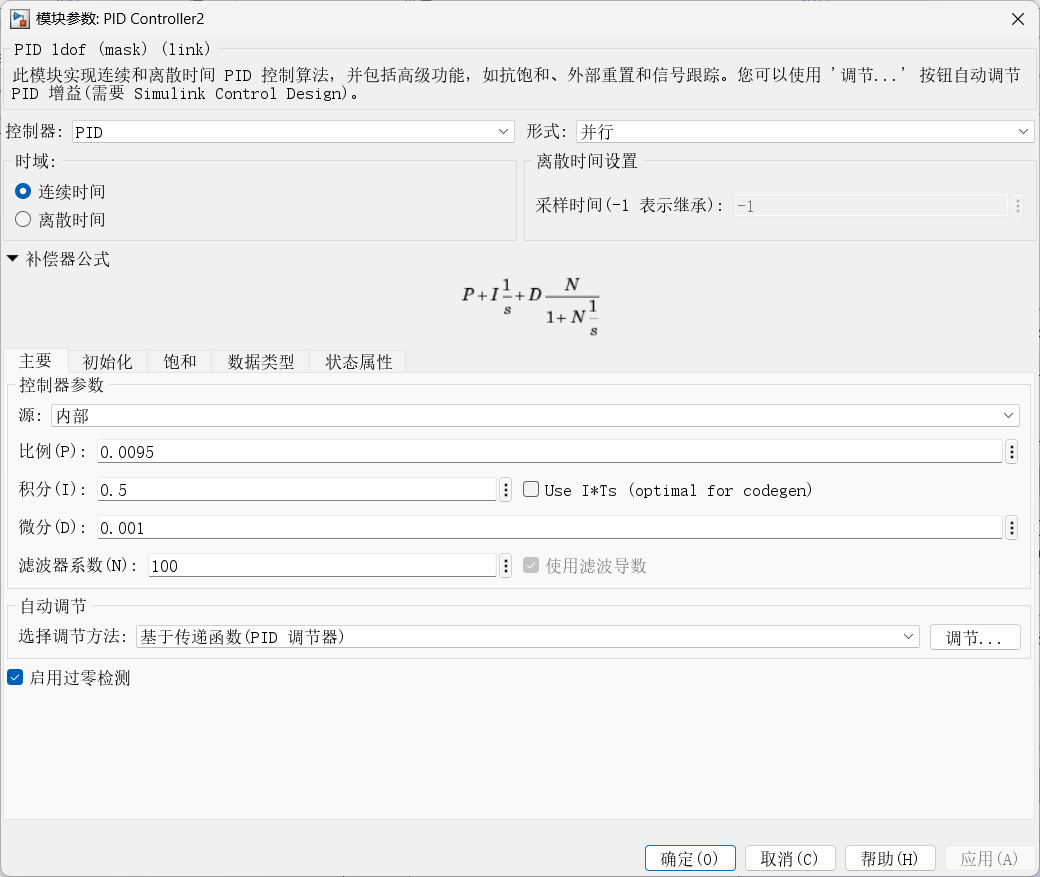
\includegraphics[width=0.3\textwidth]{2024-12-30-11-52-12.png} \caption{PID参数}\end{figure}

\subsection{Control System Designer进行自动调参}

手动调参基于试错法,需要反复调整参数,耗时耗力。

使用Control System Designer进行自动调参,可以大大提高调参效率。

这里我学习了Control System Designer的使用方法,并使用它对PID参数进行了自动调参。

\begin{figure}[htbp] \centering 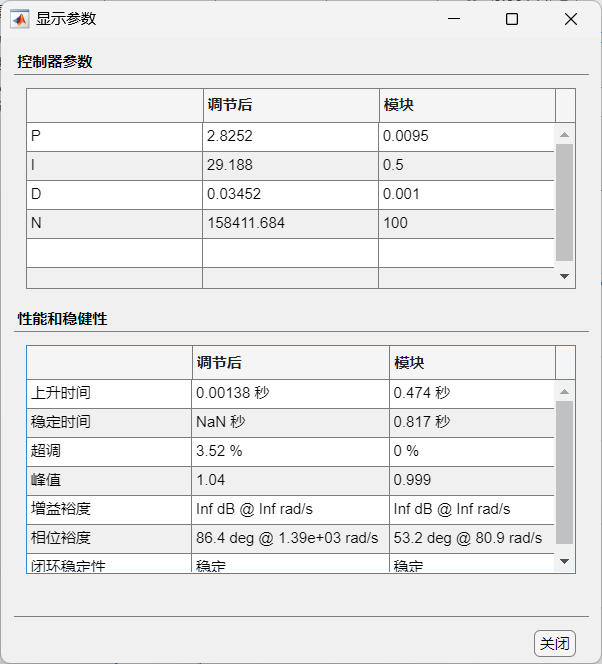
\includegraphics[width=0.3\textwidth]{2024-12-30-11-56-41.png} \caption{Control System Designer自动调参}\end{figure}

\begin{figure}[htbp] \centering 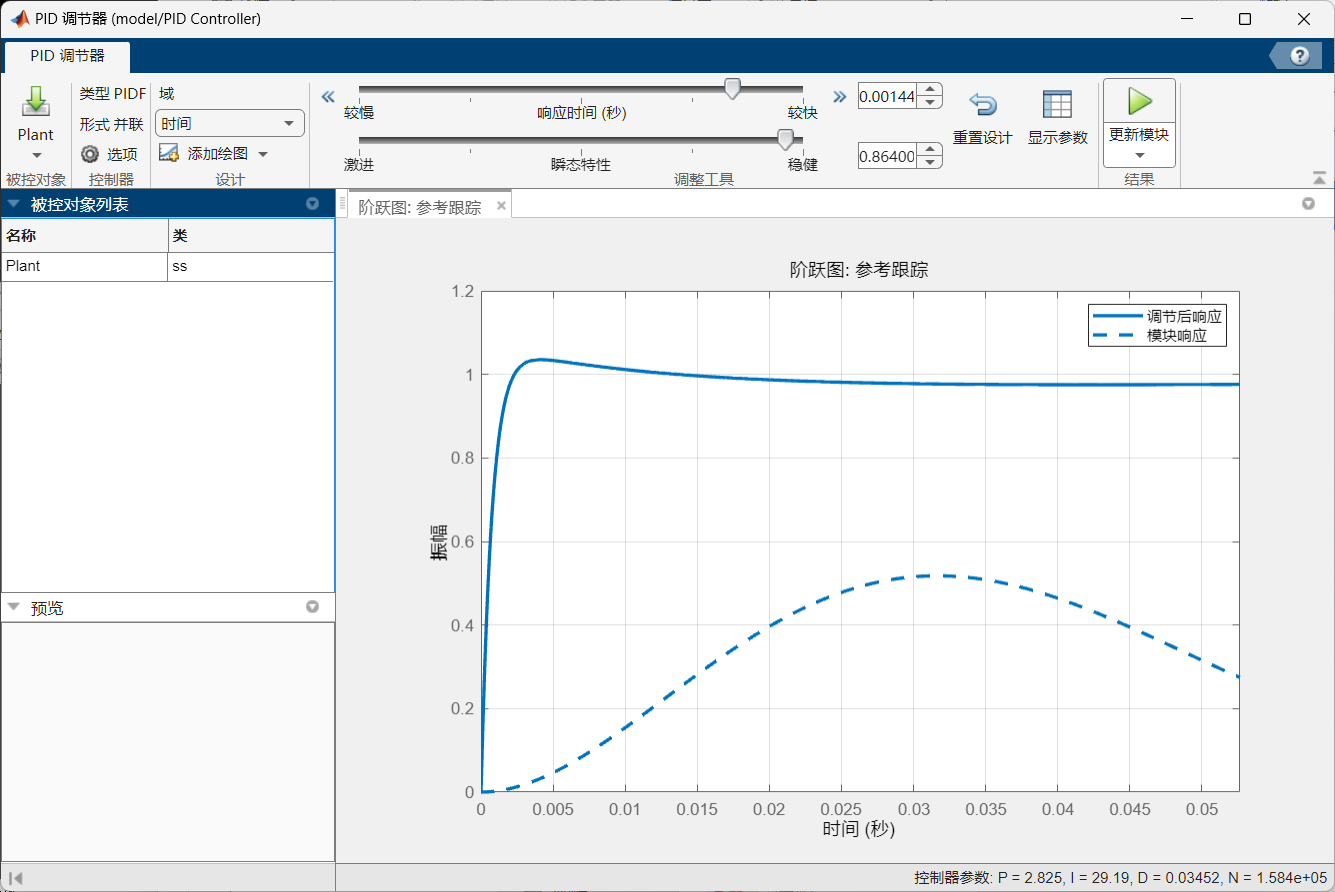
\includegraphics[width=0.4\textwidth]{2024-12-30-11-56-53.png} \caption{Control System Designer自动调参结果}\end{figure}

我发现自动调参中,使用了一些PID控制器的改进方法,比如积分限幅,使用低通滤波器,这些方法可以有效抑制超调和震荡,提高系统的稳定性。

\begin{figure}[htbp] \centering 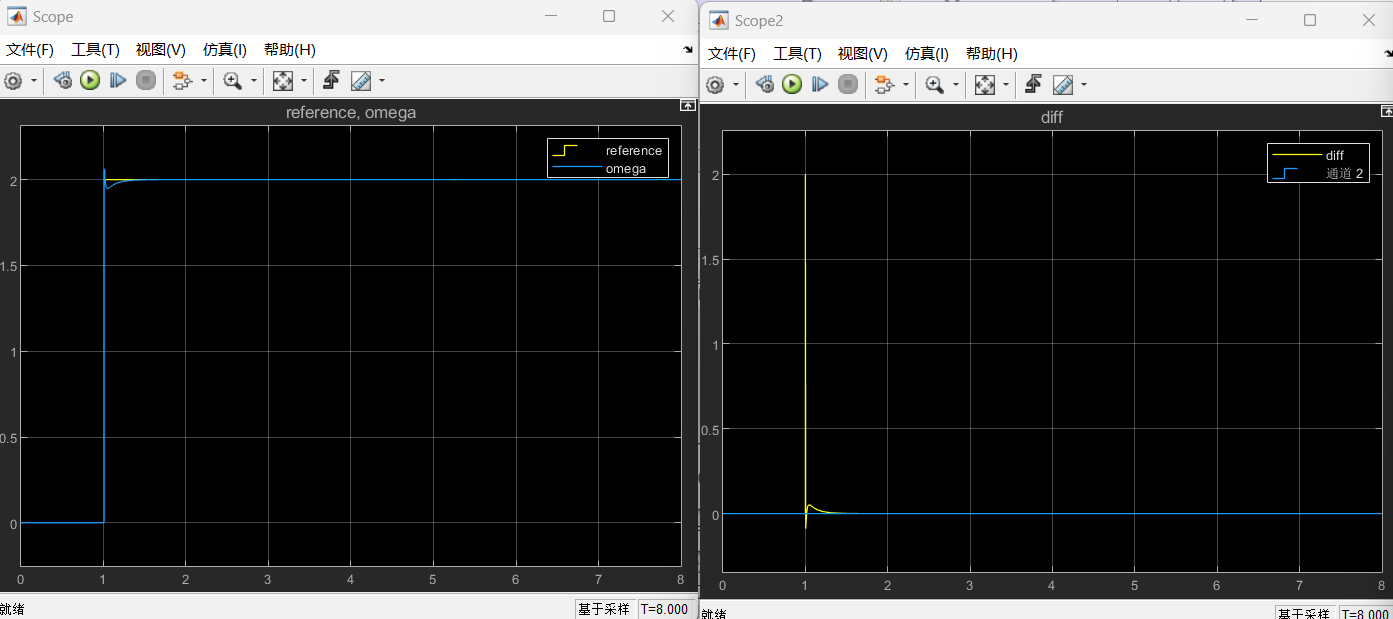
\includegraphics[width=0.7\textwidth]{2024-12-30-11-59-15.png} \caption{更改后的波形}\end{figure}

但是也需要注意的是,自动调参虽然可以调节出一个比较好的曲线,但是有时候自动调参调节出的参数的输出值会超出输入电压的范围,导致系统无法正常工作。也就是没有办法物理实现,所以在自动调参的时候,我们需要对输出值进行限幅,确保输出值在输入电压的范围之内。

\clearpage
\section{MPC模型预测控制}
\subsection{MPC控制器简介}
在秋学期的《空中机器人》课程当中,高飞老师也简要介绍了一下MPC控制器,于是,在本次大作业的过程当中,借助matlab的Control System Designer工具,我尝试设计了一个MPC控制器,并进行了仿真。

模型预测控制(Model Predictive Control, MPC)是一种先进的控制策略,它通过在线优化来预测和控制系统的未来行为。MPC的核心思想是利用系统模型在有限时域内预测系统的输出响应,并通过求解优化问题来获得最优控制序列。

MPC控制器的主要特点包括:

\begin{itemize}
\item \textbf{固定预测时域}: 在每个采样时刻,MPC都会基于当前状态,预测未来固定长度N个时间步内的系统行为。这个N称为预测时域(Prediction Horizon)。

\item \textbf{滚动优化}: 虽然MPC会计算未来N个时间步的控制序列,但只执行第一个控制量,然后在下一个采样时刻重新进行优化计算。这种方式也被称为"开环最优反馈"或"反应式规划"。

\item \textbf{在线优化}: MPC通过求解一个实时优化问题来获得控制序列,优化目标通常包括跟踪误差最小化,控制输入的平滑性,能量消耗
\end{itemize}

MPC控制器具有多方面的优势:它能够显式考虑未来时域内的系统行为,可以有效处理多变量耦合系统,能够自然地处理系统约束,同时还可以处理非线性系统和时变系统。这些特点使得MPC控制器在实际工程应用中具有很强的适用性和优越性。


\subsection{MPC控制器设计}

\begin{figure}[htbp]
    \centering
    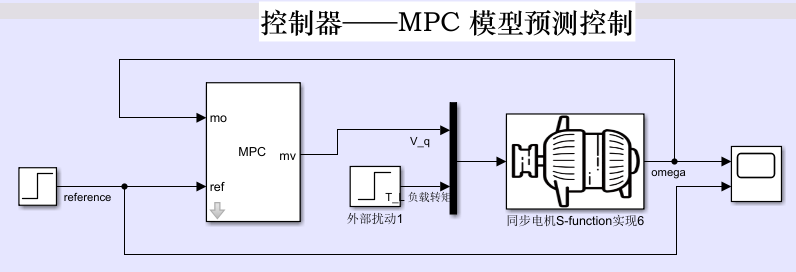
\includegraphics[width=0.6\textwidth]{20241230093059.png}
    \caption{Simulink模型}
\end{figure}
\begin{enumerate}
\item 安装MPC Designer工具箱
\item 在Simulink中建立系统模型
\item 打开设计界面,点击MPC Structure,设置输入输出通道,打开I/O Attributes,设置输入输出名称
\item 点击Update and Simulate进行仿真
\end{enumerate}

\begin{figure}[htbp]
    \centering
    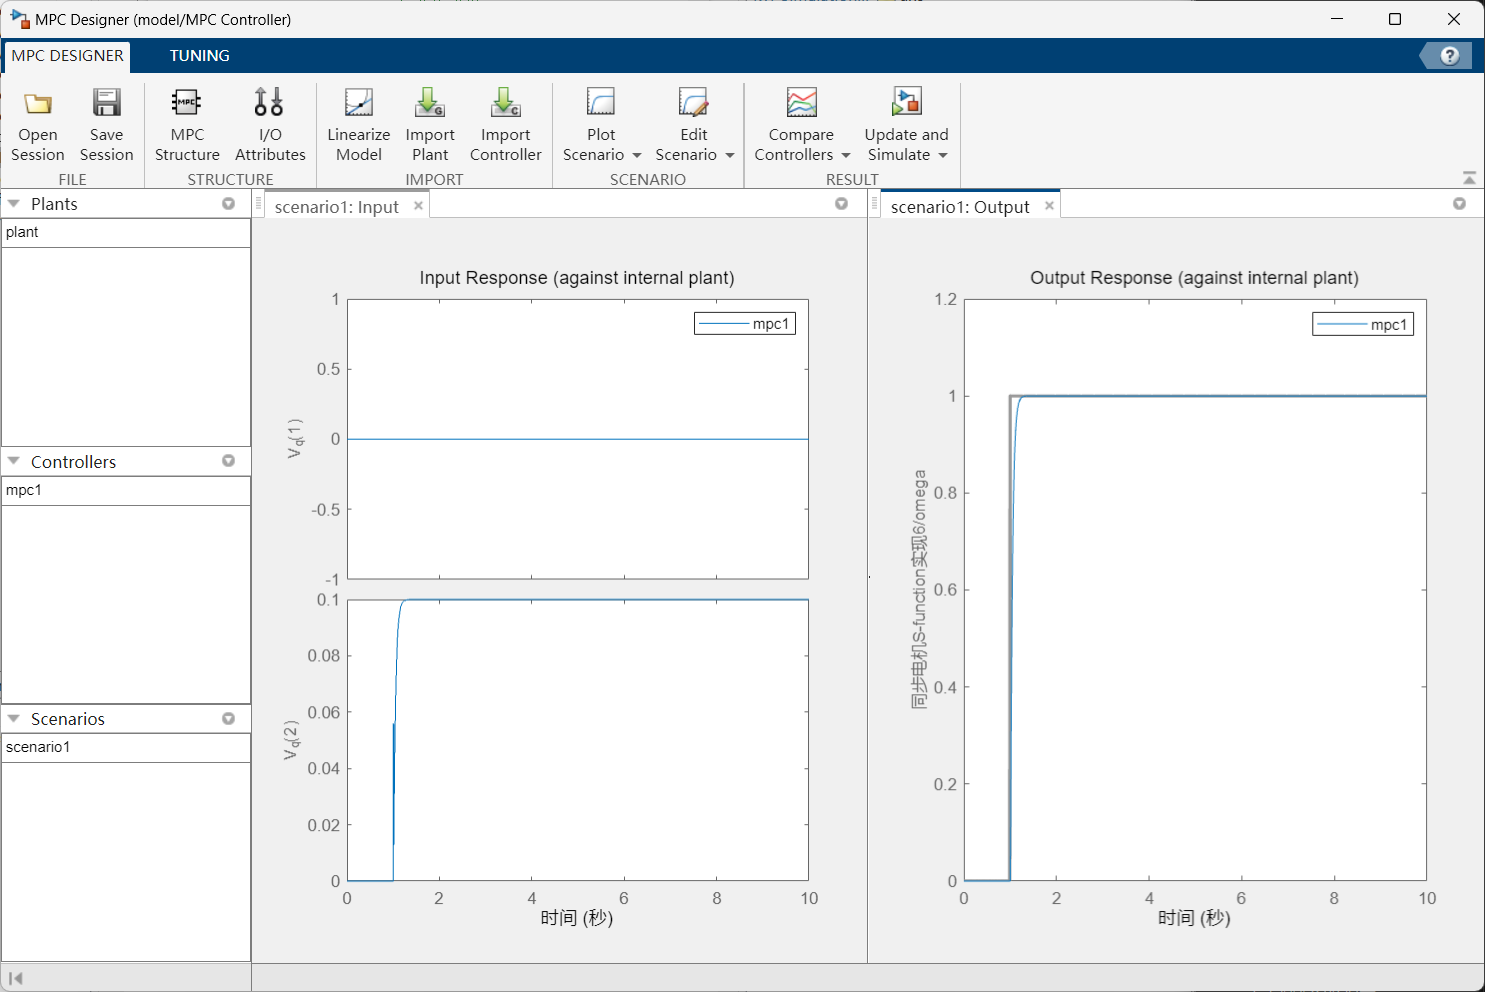
\includegraphics[width=0.8\textwidth]{20241230093026.png}
    \caption{MPC Designer设置界面}
\end{figure}

在这一部分我主要参考了以下资料:
\begin{itemize}
\item Matlab官方MPC Toolbox文档\footnote{\url{https://ww2.mathworks.cn/help/mpc/gs/introduction.html}}
\item CSDN博客《模型预测控制-Matlab自带MPC Designer工具》\footnote{\url{https://blog.csdn.net/weixin_43470383/article/details/134227287}}
\end{itemize}

\begin{lstlisting}[language=Matlab,caption=MPC控制器设计]
load('MPC_plant.mat'); % 加载模型文件
load('MPC_RefSignal.mat');
load('MPC_MDSignal.mat');
%% create MPC controller object with sample time
mpc1 = mpc(plant_C, 0.01);
%% specify prediction horizon
mpc1.PredictionHorizon = 10;
%% specify control horizon
mpc1.ControlHorizon = 2;
%% specify nominal values for inputs and outputs
mpc1.Model.Nominal.U = [0;0];
mpc1.Model.Nominal.Y = 0;
%% specify weights
mpc1.Weights.MV = [0 0];
mpc1.Weights.MVRate = [0.1 0.1];
mpc1.Weights.OV = 1;
mpc1.Weights.ECR = 100000;
%% specify simulation options
options = mpcsimopt();
options.RefLookAhead = 'off';
options.MDLookAhead = 'off';
options.Constraints = 'on';
options.OpenLoop = 'off';
%% run simulation
sim(mpc1, 1001, mpc1_RefSignal, mpc1_MDSignal, options);
\end{lstlisting}

导入到simulink中,发现其控制效果还是很好的。

\begin{figure}[htbp] \centering 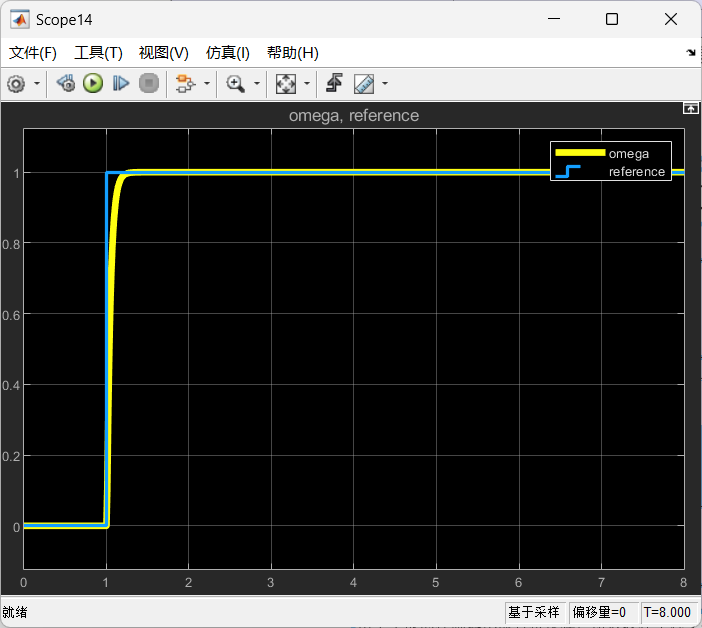
\includegraphics[width=0.6\textwidth]{2024-12-30-12-14-05.png} \caption{MPC控制器仿真结果}\end{figure}

\clearpage
\section{模糊控制}

\textbf{模糊控制的定义}
\begin{itemize}
    \item 是将模糊数学理论应用于自动控制领域的控制方法
    \item 基于模糊集合理论、模糊语言变量及模糊逻辑推理
\end{itemize}

\textbf{工作原理}
\begin{itemize}
    \item 通过观察过程输出精确量转化为模糊量
    \item 经过人脑思维与逻辑推理进行模糊判决
    \item 将判决结果的模糊量转化为精确量
\end{itemize}

\textbf{控制特性}
\begin{itemize}
    \item 属于非线性控制
    \item 不依赖于控制对象的精确模型
    \item 仅依靠少量控制规则
    \item 具有较强的鲁棒性
    \item 适用于数学模型未知、复杂的非线性系统控制
\end{itemize}


\subsection{模糊控制器设计}

根据系统逻辑,将系统slx模型搭建如下

\begin{figure}[htbp] \centering 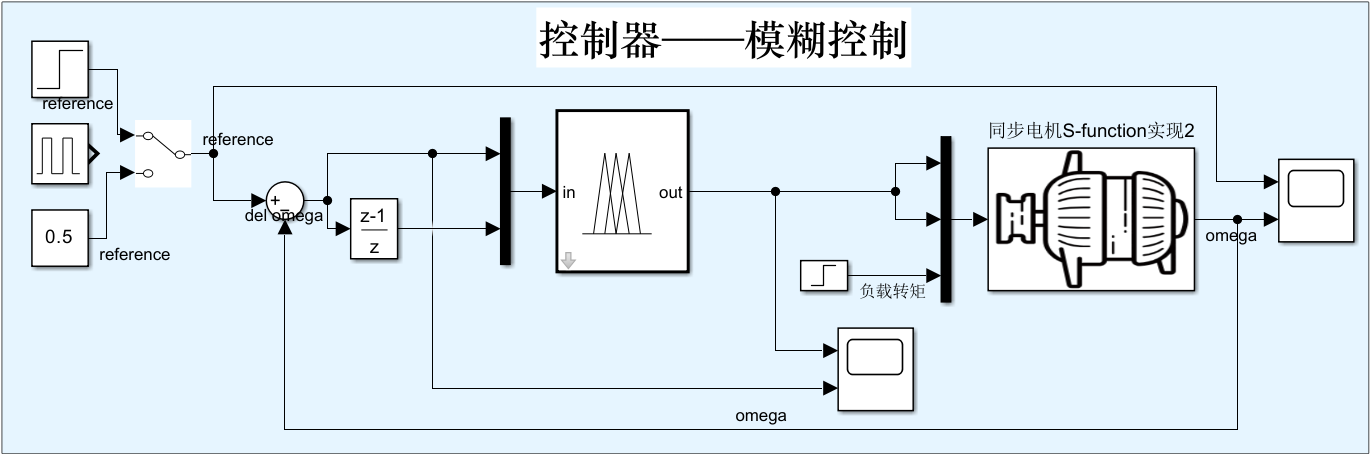
\includegraphics[width=0.7\textwidth]{2025-01-10-17-36-52.png} \caption{模糊控制器Simulink结构}\end{figure}

使用代码建立规则和隶属度函数。

$x$,$v$和$U$我都设置的是三角函数

\begin{figure}[htbp] \centering 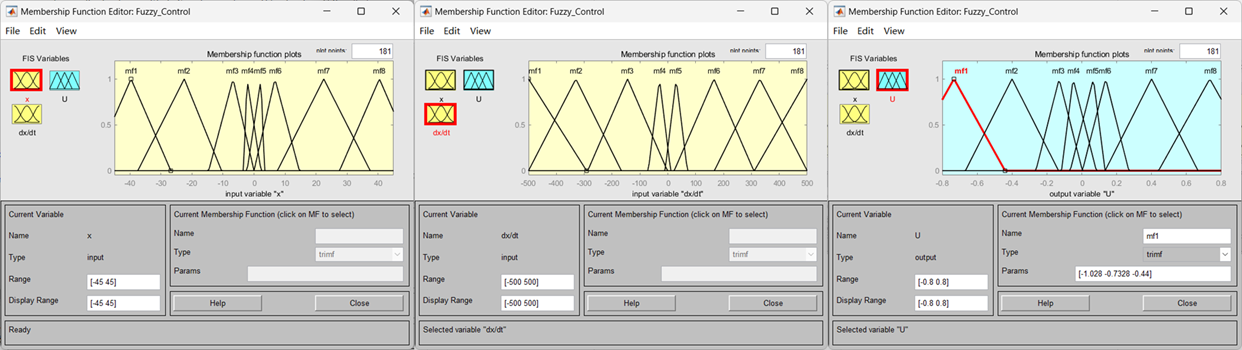
\includegraphics[width=0.7\textwidth]{2025-01-10-16-16-42.png} \caption{输入输出论域的范围}\end{figure}


\begin{lstlisting}
clear;
close all;

% 创建模糊推理系统,使用 newfis
fuzzyController = mamfis( ...
    'NumInputs',1,'NumInputMFs',2,...
    'NumOutputs',1,'NumOutputMFS',2,...
    'AddRule','none');

% 定义输入变量x(位置误差)及其隶属度函数,范围 [-0.04, 0.04]
fuzzyController.Inputs(1).Name = 'x';
fuzzyController.Inputs(1).Range = [-0.04 0.04];

fuzzyController = addMF(fuzzyController, 'input', 1, 'EN', 'trimf', [-0.05 -0.04 -0.03]); % EN: Extremely Negative
fuzzyController = addMF(fuzzyController, 'input', 1, 'VN', 'trimf', [-0.04 -0.03 -0.02]); % VN: Very Negative
fuzzyController = addMF(fuzzyController, 'input', 1, 'N', 'trimf', [-0.03 -0.02 -0.01]);  % N: Negative
fuzzyController = addMF(fuzzyController, 'input', 1, 'NZ', 'trimf', [-0.02 -0.01 0]); % Z: Zero
fuzzyController = addMF(fuzzyController, 'input', 1, 'PZ', 'trimf', [0 0.01 0.02]);  % Z: Zero
fuzzyController = addMF(fuzzyController, 'input', 1, 'P', 'trimf', [0.01 0.02 0.03]);   % P: Positive
fuzzyController = addMF(fuzzyController, 'input', 1, 'VP', 'trimf', [0.02 0.03 0.04]);  % VP: Very Positive
fuzzyController = addMF(fuzzyController, 'input', 1, 'EP', 'trimf', [0.03 0.04 0.05]);  % EP: Extremely Positive

% 可视化x的隶属度函数
figure;
subplot(311);
plotmf(fuzzyController, 'input', 1);
title('位置误差 (x) 的隶属度函数');

% 定义输入变量dx/dt(位置误差变化率)及其隶属度函数,范围 [-0.5, 0.5]
fuzzyController.Inputs(2).Name = 'dx';
fuzzyController.Inputs(2).Range = [-0.5 0.5];
fuzzyController = addMF(fuzzyController, 'input', 2, 'EN', 'trimf', [-0.6 -0.5 -0.4]);  % EN: Extremely Negative
fuzzyController = addMF(fuzzyController, 'input', 2, 'VN', 'trimf', [-0.5 -0.4 -0.3]);  % VN: Very Negative
fuzzyController = addMF(fuzzyController, 'input', 2, 'N', 'trimf', [-0.4 -0.3 -0.2]);  % N: Negative
fuzzyController = addMF(fuzzyController, 'input', 2, 'NZ', 'trimf', [-0.2 -0.1 0]);     % Z: Zero
fuzzyController = addMF(fuzzyController, 'input', 2, 'PZ', 'trimf', [0 0.1 0.2]);     % Z: Zero
fuzzyController = addMF(fuzzyController, 'input', 2, 'P', 'trimf', [0.2 0.3 0.4]);   % P: Positive
fuzzyController = addMF(fuzzyController, 'input', 2, 'VP', 'trimf', [0.3 0.4 0.5]);   % VP: Very Positive
fuzzyController = addMF(fuzzyController, 'input', 2, 'EP', 'trimf', [0.4 0.5 0.6]);   % EP: Extremely Positive

% 可视化dx/dt的隶属度函数
subplot(312);
plotmf(fuzzyController, 'input', 2);
title('位置误差变化率 (dx/dt) 的隶属度函数');

% 定义输出变量U(控制电压)的隶属度函数,范围 [-10, 10]
fuzzyController = addvar(fuzzyController, 'output', 'U', [-10 10]);
fuzzyController = addMF(fuzzyController, 'output', 1, 'EL', 'trimf', [-10 -10 -7]);  % EL: Extremely Low
fuzzyController = addMF(fuzzyController, 'output', 1, 'VL', 'trimf', [-10 -7 -4]);  % VL: Very Low
fuzzyController = addMF(fuzzyController, 'output', 1, 'L', 'trimf', [-7 -4 -1]);   % L: Low
fuzzyController = addMF(fuzzyController, 'output', 1, 'NZ', 'trimf', [-3 -1 1]);  % NZ:negetive ZERO
fuzzyController = addMF(fuzzyController, 'output', 1, 'PZ', 'trimf', [-1 1 3]);  % M: positive ZERO
fuzzyController = addMF(fuzzyController, 'output', 1, 'H', 'trimf', [1 4 7]);  % H: High
fuzzyController = addMF(fuzzyController, 'output', 1, 'VH', 'trimf', [4 7 10]); % VH: Very High
fuzzyController = addMF(fuzzyController, 'output', 1, 'EH', 'trimf', [7 10 10]); % EH: Extremely High
\end{lstlisting}

但是值得注意的是,根据调试信息可以看出,这种方法已经逐步被淘汰了,在接下来的版本当中将全被替换成为ui界面操作

\subsubsection{模糊规则的设计}
其实使用代码生成模糊矩阵比手动一个个点还是要快一些的,这也是我为什么选择这种方法的原因。


这里我使用了另一个课本中给出的一个参考8x8矩阵作为调参的backbone,之后我在这个的基础上进行了对于我这个系统的调参和修改。


\begin{lstlisting}[language=Matlab,caption=生成规则矩阵]
fuzzyController = readfis('Fuzzy_Control.fis');

table = [
    [1, 1, 1, 1, 6, 5, 5, 5],
    [1, 2, 2, 1, 7, 5, 5, 5],
    [2, 2, 2, 1, 2, 6 ,6, 6],
    [2, 3, 3, 2, 7, 6, 6, 6],
    [3, 3, 3, 2, 8, 7, 6, 7],
    [3, 3, 4, 2,8, 7, 7, 7],
    [3, 4, 4, 2, 8, 8, 7, 8],
    [4, 4, 4, 4, 8, 8, 8, 8]];
% 生成规则矩阵
rules = [];
for i = 1:8
    for j = 1:8
        disp(table(i,j));
        output = table(i,j);
        rules = [rules; i j  output 1 1]; % 1 1表示使用 'min' 合成和 'centroid' 解模糊
    end
end

% disp(rules)

% 添加规则到模糊系统
fuzzyController = addrule(fuzzyController, rules);
%showrule(fuzzyController,'Format','symbolic');
\end{lstlisting}



\begin{lstlisting}[language=Matlab,caption=可视化规则]
% 可视化规则
ruleview(fuzzyController);

%figure;
%plotfis(fuzzyController);

% 输出 surface
figure;
gensurf(fuzzyController,[1,2],1);
saveas(gcf, 'surf.jpg');

% 保存为.fis文件
writefis(fuzzyController, 'Fuzzy_Control.fis');
\end{lstlisting}

建立了初步的规则,但在系统上进行尝试的时候发现效果并不好,经常会出现不收敛、不稳定、震荡大等问题。

所以经过反复多次的修改和尝试,最后得到了一版规则,可以达到给定的效果。


\begin{figure}[htbp] \centering 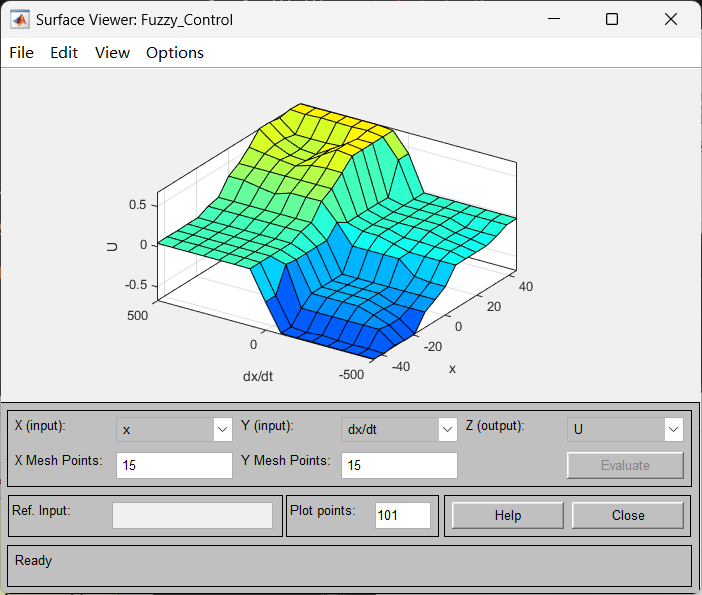
\includegraphics[width=0.4\textwidth]{2025-01-10-16-18-48.png} \caption{模糊控制surface的形状}\end{figure}

\subsubsection{模糊控制器调参效果}

\begin{figure}[htbp] \centering 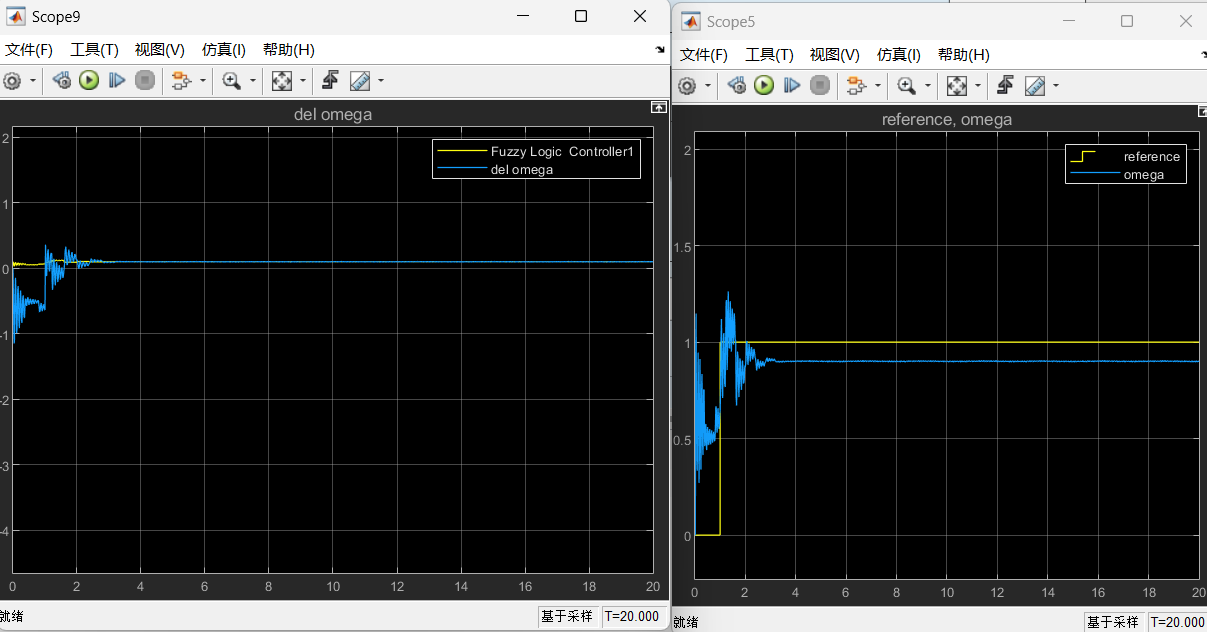
\includegraphics[width=0.7\textwidth]{2025-01-10-13-42-51.png} \caption{第一次调参后,不能稳定在参考输入上}\end{figure}

\begin{figure}[htbp] \centering 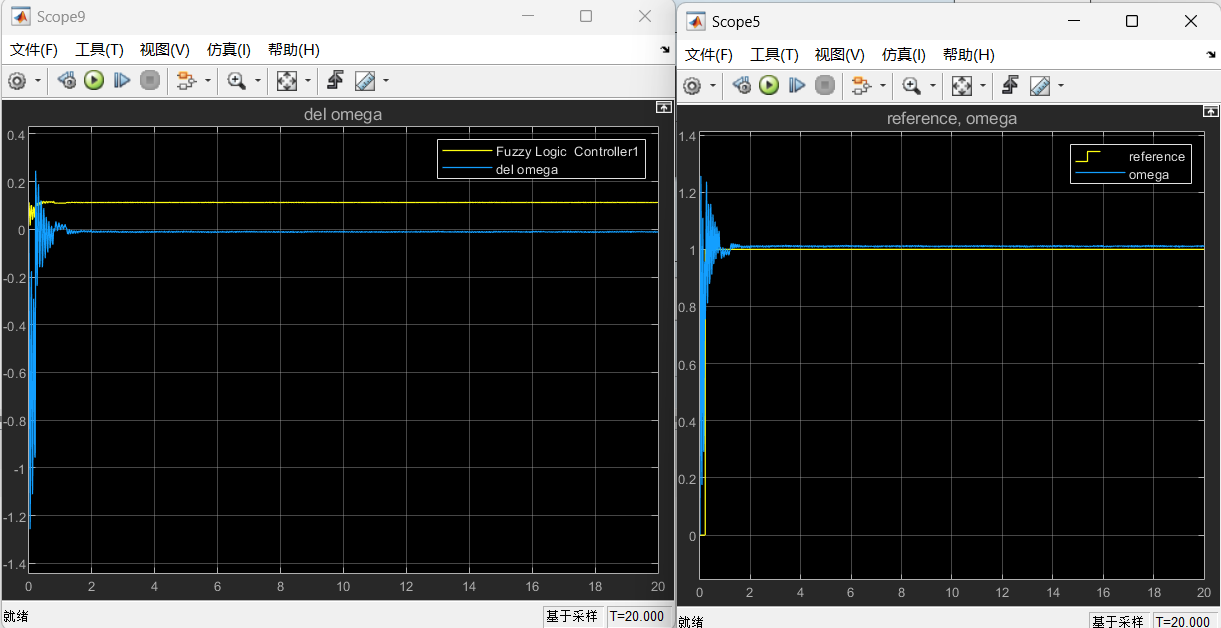
\includegraphics[width=0.7\textwidth]{2025-01-10-13-45-18.png} \caption{第二次调参后,稳定在阶跃输入上}\end{figure}

从上面的仿真结果可以看出:

\begin{enumerate}
\item 系统响应性能良好。从图中可以看出,系统能够快速跟踪给定的参考输入信号,位置误差在短时间内就能收敛到参考位置附近。

\item 稳态精度合理。在稳态时,位置x能够很好地跟随参考输入,稳态误差比较小,满足控制要求。
\end{enumerate}
\newpage
\subsection{模糊PID控制}

\begin{figure}[htbp] \centering 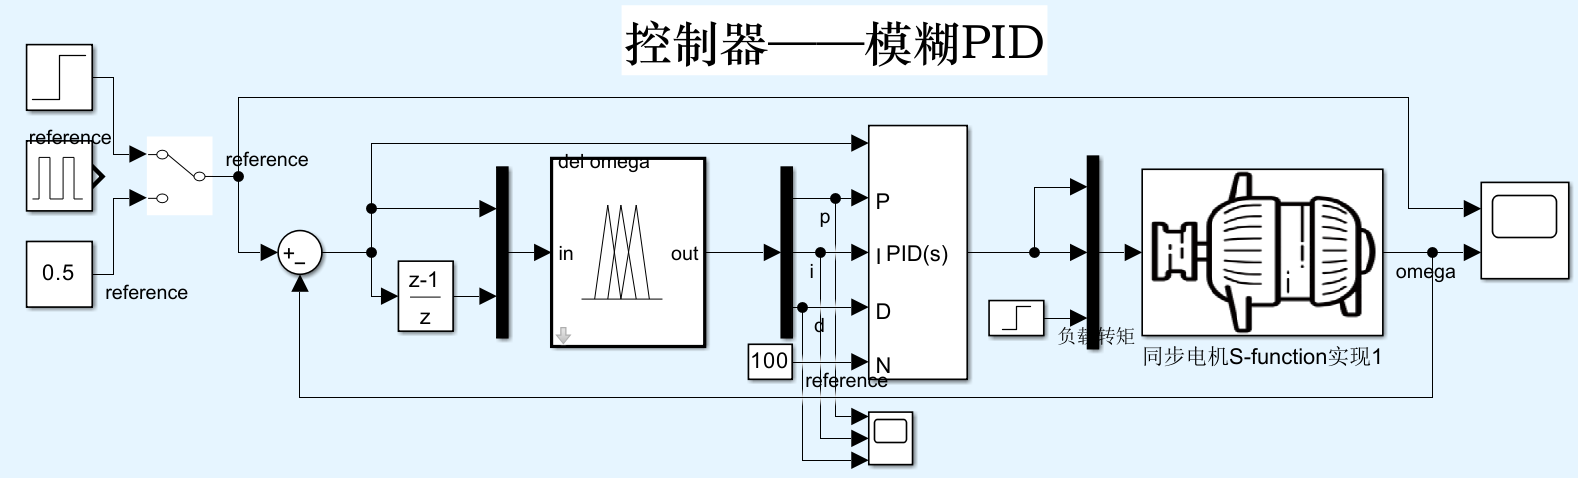
\includegraphics[width=0.7\textwidth]{2024-12-30-12-22-09.png} \caption{模糊PID Simulink结构}\end{figure}

模糊PID控制器是将模糊控制和PID控制相结合的一种智能控制方法。它利用模糊控制的专家经验来在线调整PID控制器的参数,从而提高系统的控制性能。

在永磁同步电机的速度控制中,模糊PID控制器以速度误差$e$和误差变化率$ec$作为输入,通过模糊推理得到PID参数的调整量$\Delta K_p$、$\Delta K_i$和$\Delta K_d$。具体工作过程如下:

\begin{enumerate}
\item 首先将速度误差$e$和误差变化率$ec$进行模糊化,即将精确值映射到相应的模糊集合中。
\item 根据专家经验建立模糊规则库,描述$e$和$ec$与PID参数调整量之间的关系。
\item 采用模糊推理得到$\Delta K_p$、$\Delta K_i$和$\Delta K_d$的模糊值。
\item 对模糊推理结果进行解模糊化,得到PID参数的具体调整量。
\end{enumerate}


所以,根据以下的论域范围和隶属度函数,我设计了一个模糊控制的PID


\begin{figure}[htbp] \centering 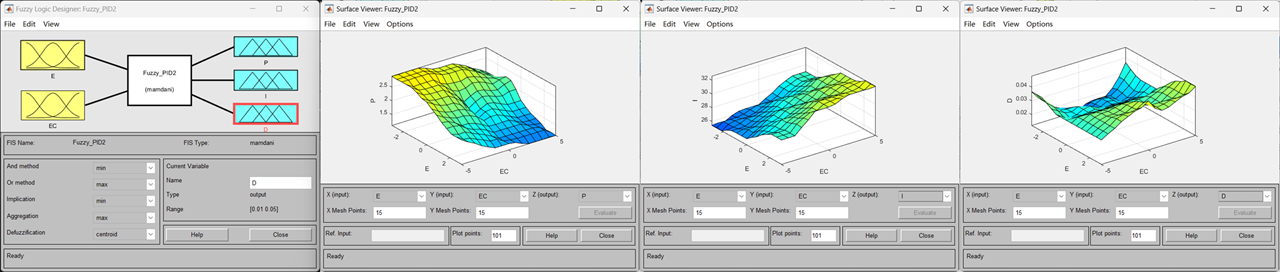
\includegraphics[width=\textwidth]{2024-12-30-12-30-02.png} \caption{模糊PID论域范围与决策平面}\end{figure}


\begin{figure}[htbp] \centering 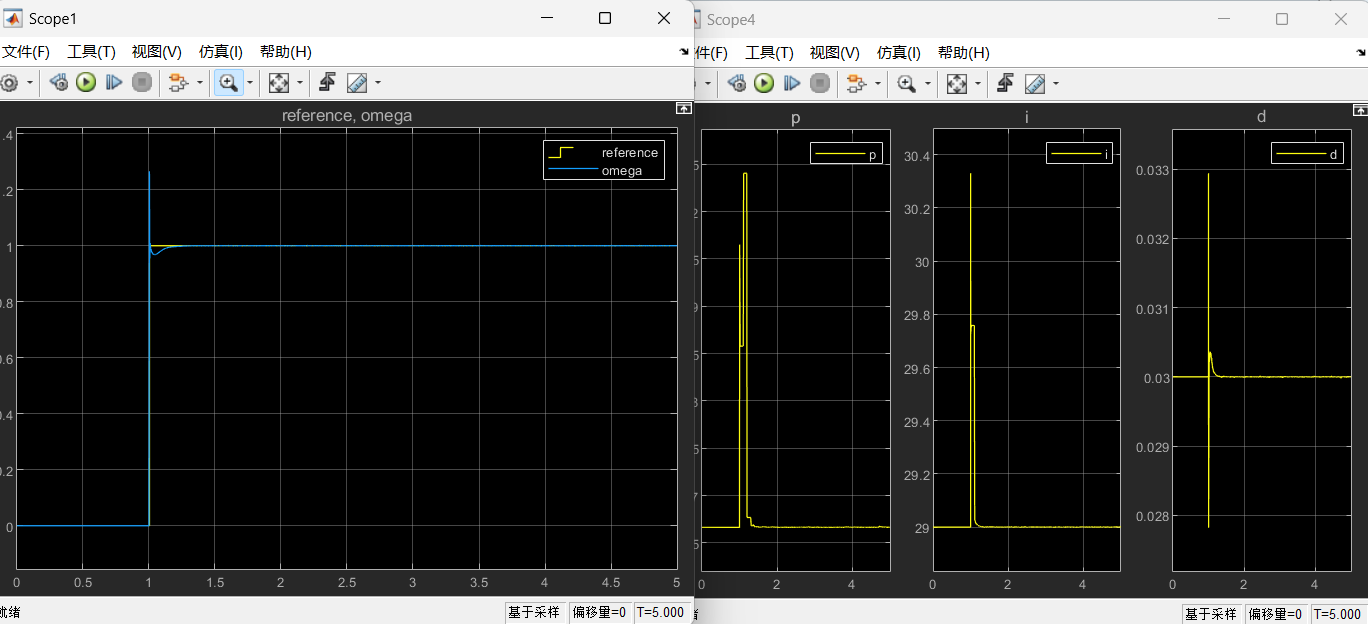
\includegraphics[width=0.7\textwidth]{2024-12-30-12-27-30.png} \caption{模糊PID控制器}\end{figure}

这个初版的结果并不理想,所以我对论域范围和规则进行了调整,得到了以下结果


\clearpage
\section{神经网络建模控制}

\subsection{BP-PID控制}

第二种方法是基于BP神经网络的PID控制
经典的增量式数字PID控制算法的公式为:

\begin{equation}
u(k) = u(k-1) + K_p[e(k) - e(k-1)] + K_i e(k) + K_d[e(k) - 2e(k-1) + e(k-2)]
\end{equation}

其中:
\begin{itemize}
\item $u(k)$ 是当前采样时刻的控制量
\item $e(k)$ 是当前采样时刻的期望输出与实际输出之差
\item $K_p$、$K_i$、$K_d$ 分别是比例、积分、微分系数
\end{itemize}

\begin{figure}[htbp] \centering 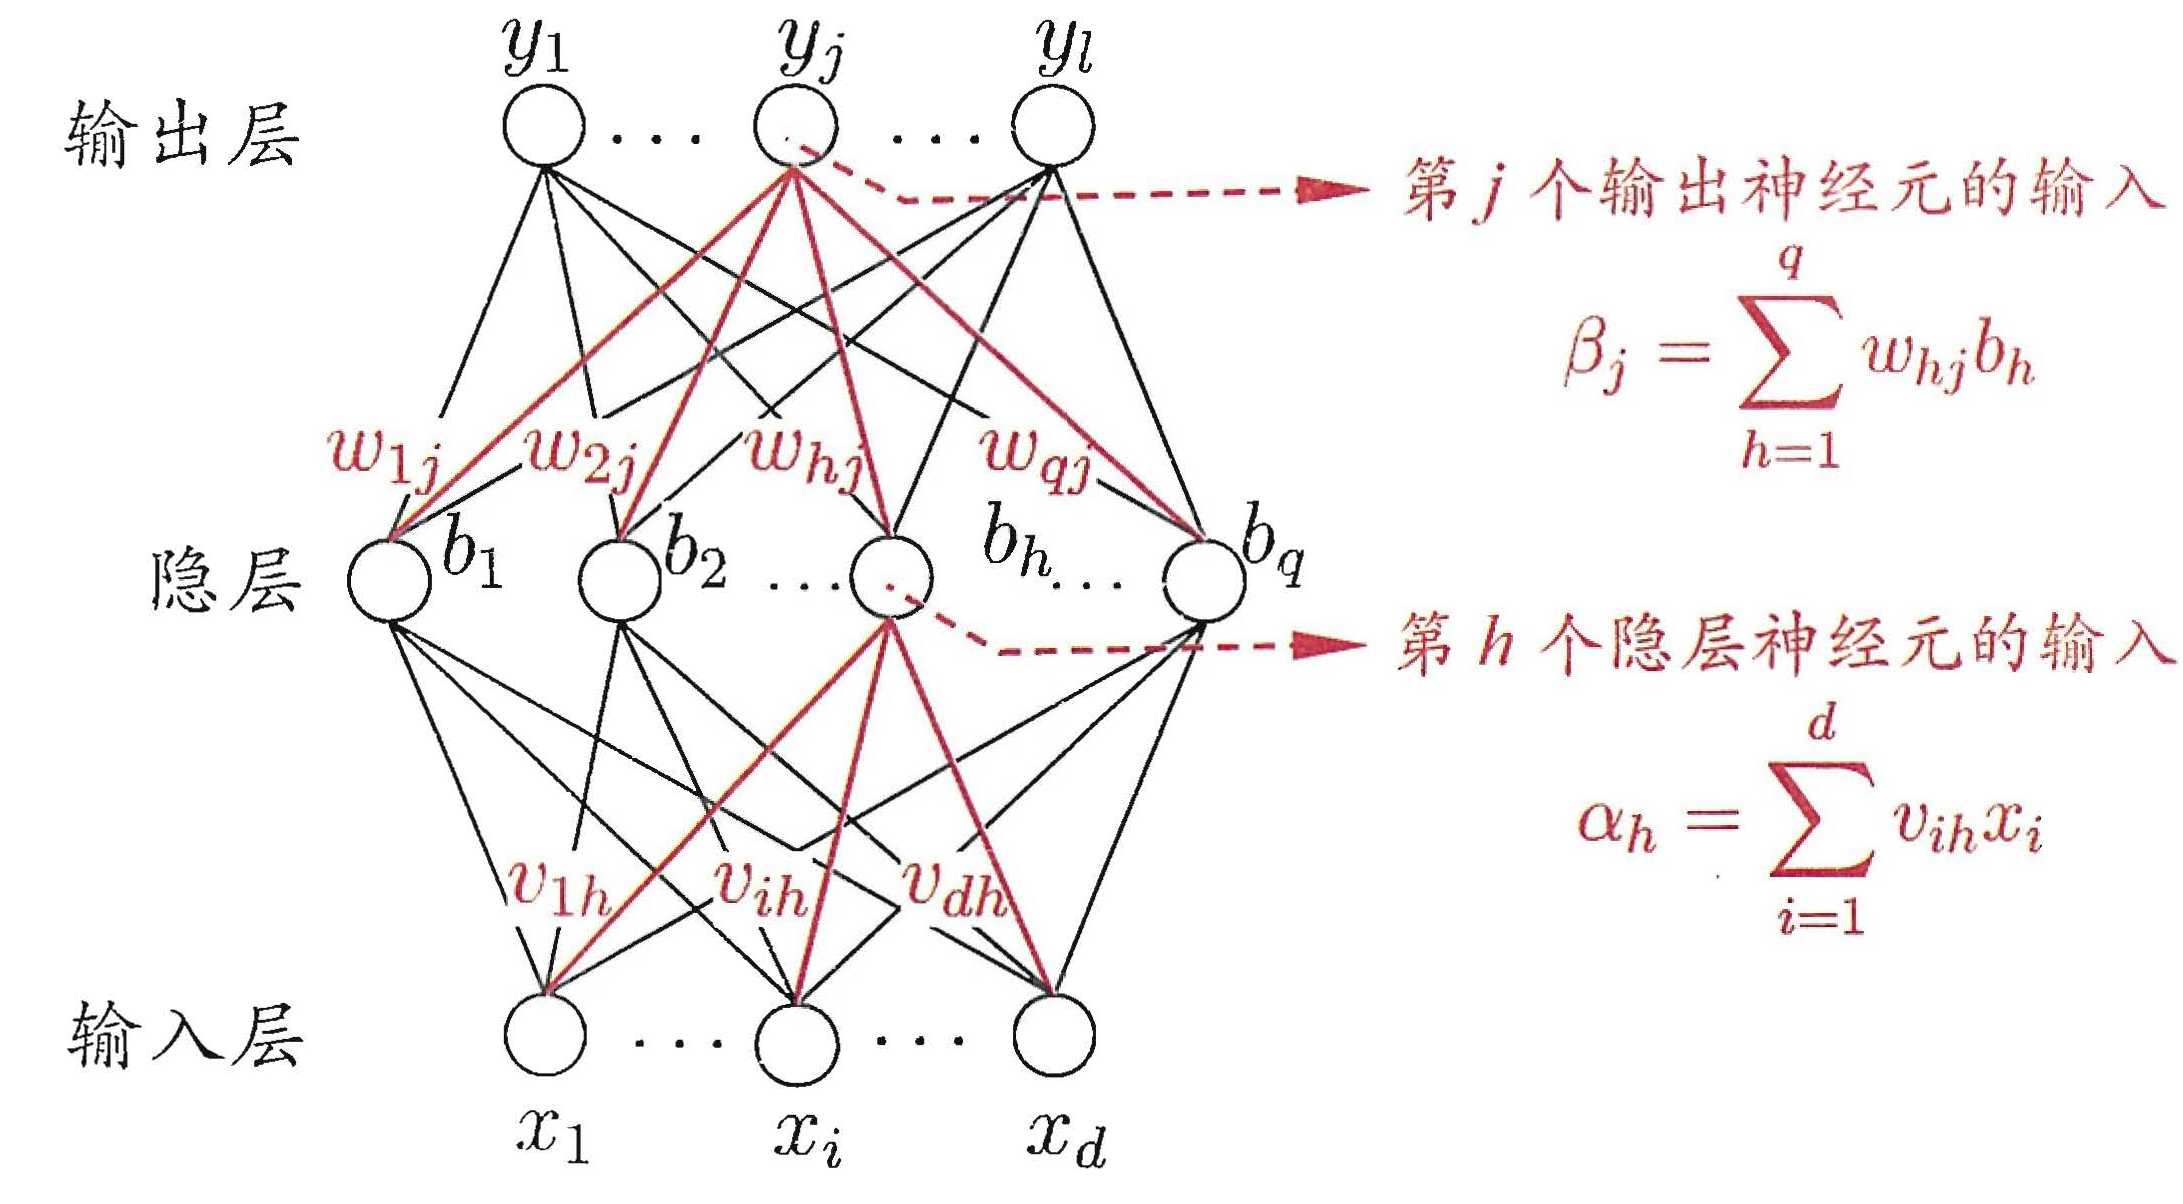
\includegraphics[width=0.7\textwidth]{2024-12-30-13-31-18.png} \caption{BP-PID控制器结构}\end{figure}

将 $K_p$、$K_i$、$K_d$ 视为依赖于系统运行状态的可调参数时,可以将上述描述表示为:

\begin{equation}
u(k) = f[u(k-1), K_p, K_i, K_d, e(k), e(k-1), e(k-2)]
\end{equation}

其中,$f(\cdot)$ 是一个与 $K_p$、$K_i$、$K_d$、$u(k-1)$、$e(k)$ 等有关的非线性函数。这个函数可以通过训练和学习来找到最佳的控制规律,通常使用BP神经网络(反向传播神经网络)来实现。

包括输入层、隐含层和输出层。输出层的三个输出分别对应PID控制器的三个可调参数$K_p$、$K_i$和$K_d$。由于这些参数不能为负,所以输出层神经元的变换函数选择非负的Sigmoid函数。

\begin{figure}[htbp] \centering 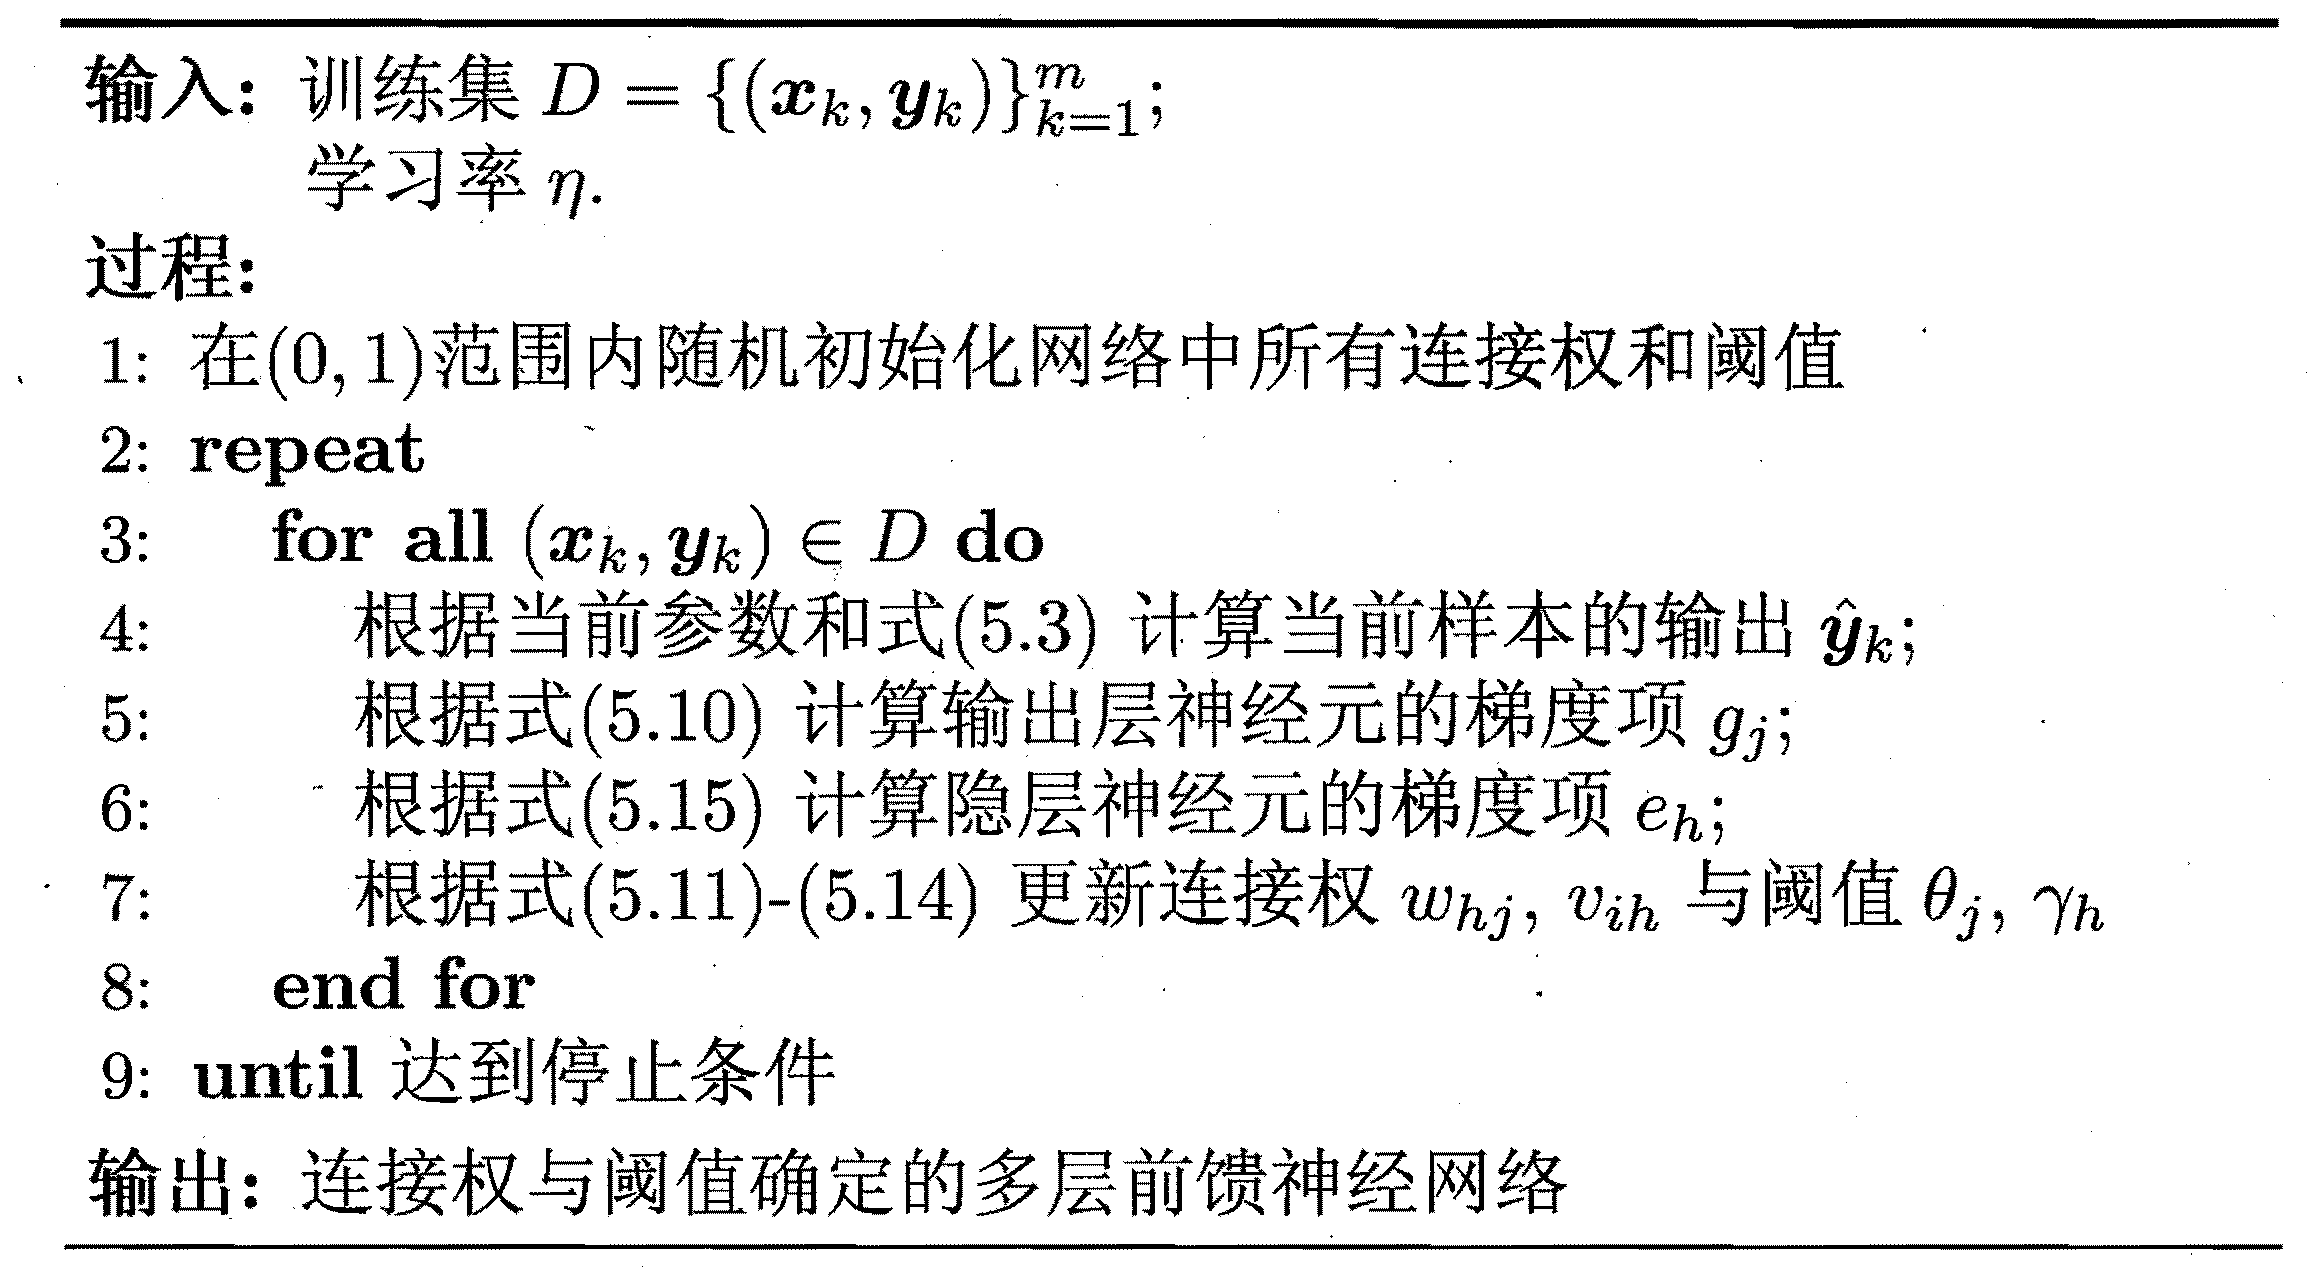
\includegraphics[width=0.7\textwidth]{2024-12-30-13-30-41.png} \caption{BP算法流程 —— 图源《机器学习 周志华》}\end{figure}

所以,根据这样的结构,我设计了BP-PID控制器,并使用simulink进行了仿真。


\begin{lstlisting}[language=Matlab,caption=BPD-PID控制器实现]
    function [sys,x0,str,ts,simStateCompliance] = bppid(t,x,u,flag,T,nh,xite,alfa)
    % 输入参数:
    % nh: 隐含层神经元数量 (hidden_neurons)
    % xite: 学习率 (learning_rate)
    % alfa: 动量因子 (momentumfactor)
    % T: 采样时间 (sampling_time)
    % 这些参数已经使用mask方法在simulink中设置
    switch flag
        case 0
            [sys,x0,str,ts,simStateCompliance] = mdlInitializeSizes(T,nh); % 初始化函数
        case 1
            sys = mdlDerivatives(t, x, u);
        case 2
            sys = mdlUpdate(t, x, u);
        case 3
            sys = mdlOutputs(t,x,u,nh,xite,alfa); % 输出函数
        case 9
            sys = mdlTerminate(t, x, u);
        otherwise
            DAStudio.error('Simulink:blocks:unhandledFlag', num2str(flag));
    end
end

function [sys,x0,str,ts,simStateCompliance] = mdlInitializeSizes(T,nh)
    % 调用初始化函数
    % 输入参数:
    %   T  - 采样时间
    %   nh - 隐含层神经元个数
    sizes = simsizes;
    sizes.NumContStates  = 0;
    sizes.NumDiscStates  = 0;
    sizes.NumOutputs     = 4+6*nh;  % 输出维数:控制量u,PID参数(Kp,Ki,Kd),隐含层和输出层权值
    sizes.NumInputs      = 7+12*nh; % 输入维数:[e(k),e(k-1),e(k-2),y(k),y(k-1),r(k),u(k-1)],前后两次权值
    sizes.DirFeedthrough = 1;
    sizes.NumSampleTimes = 1;
    sys = simsizes(sizes);
    x0  = [];
    str = [];
    ts  = [T 0];
    simStateCompliance = 'UnknownSimState';
end

function sys = mdlOutputs(~,~,u,nh,xite,alfa)
    % 如果权值未初始化,则随机初始化
    if any(isnan(u(8:7+12*nh)))
        hiddenWeights_prev2 = 0.5 * randn(nh,3) - 0.25; % 隐含层前两次权值(k-2)
        outputWeights_prev2 = 0.5 * randn(3,nh) - 0.25; % 输出层前两次权值(k-2) 
        hiddenWeights_prev1 = 0.5 * randn(nh,3) - 0.25; % 隐含层前一次权值(k-1)
        outputWeights_prev1 = 0.5 * randn(3,nh) - 0.25; % 输出层前一次权值(k-1)
    else
        hiddenWeights_prev2 = reshape(u(8:7+3*nh),nh,3);      % 隐含层前两次权值矩阵(nh×3)
        outputWeights_prev2 = reshape(u(8+3*nh:7+6*nh),3,nh); % 输出层前两次权值矩阵(3×nh)
        hiddenWeights_prev1 = reshape(u(8+6*nh:7+9*nh),nh,3); % 隐含层前一次权值矩阵(nh×3)
        outputWeights_prev1 = reshape(u(8+9*nh:7+12*nh),3,nh);% 输出层前一次权值矩阵(3×nh)
    end
    
    % 神经网络输入
    networkInput = [u(6),u(4),u(1)];  % [r(k),y(k),e(k)]
    pidInput = [u(1)-u(2);u(1);u(1)+u(3)-2*u(2)];  % [e(k)-e(k-1);e(k);e(k)+e(k-2)-2*e(k-1)]
    
    % 计算隐含层输入
    hiddenInput = networkInput * hiddenWeights_prev1';  % 维数:1×nh
    
    % 限制隐含层输入范围,防止溢出
    for i = 1:length(hiddenInput)
        hiddenInput(i) = min(max(hiddenInput(i), -500), 500);
    end
    
    % 隐含层输出(使用Sigmoid激活函数)
    hiddenOutput = exp(hiddenInput)./(exp(hiddenInput)+exp(-hiddenInput));
    % hiddenOutput = max(0, hiddenInput);  % 可选用ReLU激活函数
    
    % 输出层计算
    outputLayerInput = outputWeights_prev1 * hiddenOutput';  % 维数:3×1
    
    % PID参数计算(使用Sigmoid导数作为激活函数)
    pidParams = 2./(exp(outputLayerInput)+exp(-outputLayerInput)).^2;
    pidParams = pidParams/100;  % 缩放PID参数
    
    % 计算控制量
    controlOutput = u(7) + pidParams' * pidInput;
    
    % 计算梯度
    gradientSign = sign((u(4)-u(5))/(controlOutput-u(7)+0.0000001));
    pidParamsGradient = 2./(exp(pidParams)+exp(-pidParams)).^2;
    
    % 下面是BP神经网络的权值更新部分
    % 计算delta项
    delta = u(1) * gradientSign * pidInput .* pidParamsGradient;
    
    % 更新权值
    outputWeights = outputWeights_prev1 + xite*delta*hiddenOutput + alfa*(outputWeights_prev1-outputWeights_prev2);
    
    % 计算隐含层梯度
    hiddenGradient = 2./(exp(hiddenOutput)+exp(-hiddenOutput)).^2;
    % hiddenGradient = double(hiddenInput > 0);  % ReLU导数
    
    % 更新隐含层权值
    hiddenWeights = hiddenWeights_prev1 + xite*(hiddenGradient.*(delta'*outputWeights))'*networkInput + alfa*(hiddenWeights_prev1-hiddenWeights_prev2);
    
    % 整合输出
    sys = [controlOutput;pidParams(:);hiddenWeights(:);outputWeights(:)];
end

function sys = mdlDerivatives(~,~,~)
    sys = [];
end

function sys = mdlUpdate(~, ~, ~)
    sys = [];
end

function sys = mdlTerminate(~, ~, ~)
    sys = [];
end
\end{lstlisting}

\textbf{BP-PID控制器计算流程}

BP-PID控制器的核心思想是使用神经网络来动态调整PID控制器的参数。整个控制器的计算过程可以分为以下几个步骤:

\textbf{神经网络结构}
\begin{itemize}
\item 输入层接收系统状态,包括参考输入\(r(k)\)、系统输出\(y(k)\)和控制误差\(e(k)\)
\item 隐含层包含\(nh\)个神经元,使用Sigmoid函数作为激活函数
\item 输出层有3个神经元,分别对应PID控制器的三个参数\(K_p\)、\(K_i\)、\(K_d\)
\end{itemize}

\textbf{前向计算过程}

网络的前向计算分为以下步骤:

1. 隐含层计算:
   \begin{equation}
   \begin{aligned}
   & \text{隐含层输入:} I = \mathbf{x}_\text{input} \cdot W_i^T \\
   & \text{隐含层输出:} O_h = \frac{\exp(I)}{\exp(I) + \exp(-I)}
   \end{aligned}
   \end{equation}

2. 输出层计算:
   \begin{equation}
   \begin{aligned}
   & \text{输出层输入:} O = W_o \cdot O_h^T \\
   & \text{PID参数:} \mathbf{K} = \frac{2}{(\exp(O) + \exp(-O))^2}
   \end{aligned}
   \end{equation}

3. 控制量计算:
   \begin{equation}
   u(k) = u(k-1) + K_p[e(k) - e(k-1)] + K_i e(k) + K_d[e(k) - 2e(k-1) + e(k-2)]
   \end{equation}

\textbf{参数使用BP算法更新}


1. 计算输出层的误差梯度:
   \begin{equation}
   \delta_o = \text{sign}\left(\frac{e(k)-e(k-1)}{u(k)-u(k-1)}\right) \cdot \frac{\partial O}{\partial K}
   \end{equation}

2. 更新输出层权重:
   \begin{equation}
   W_o^{new} = W_o + \eta \cdot \delta_o \cdot O_h + \alpha(W_o - W_o^{old})
   \end{equation}
   其中\(\eta\)是学习率,\(\alpha\)是动量因子。

3. 更新隐含层权重:
   \begin{equation}
   W_i^{new} = W_i + \eta \cdot (\delta_o \cdot W_o)^T \cdot \mathbf{x}_\text{input} + \alpha(W_i - W_i^{old})
   \end{equation}

\textbf{控制器特点}

\begin{itemize}
\item 通过神经网络的学习能力,可以自适应调整PID参数
\item 采用增量式PID算法,避免了积分饱和问题
\item 引入动量项加快收敛速度,提高控制性能
\item 使用Sigmoid函数保证PID参数始终为正值
\end{itemize}


设计了BP-PID控制器之后,我先在一阶传递函数的被控对象上进行了尝试,发现可以很好的控制。

根据图\ref{fig:one_order_system} ,可以发现子经过调整之后,找到了比较合适的PID参数。

\begin{figure}[htbp] \centering 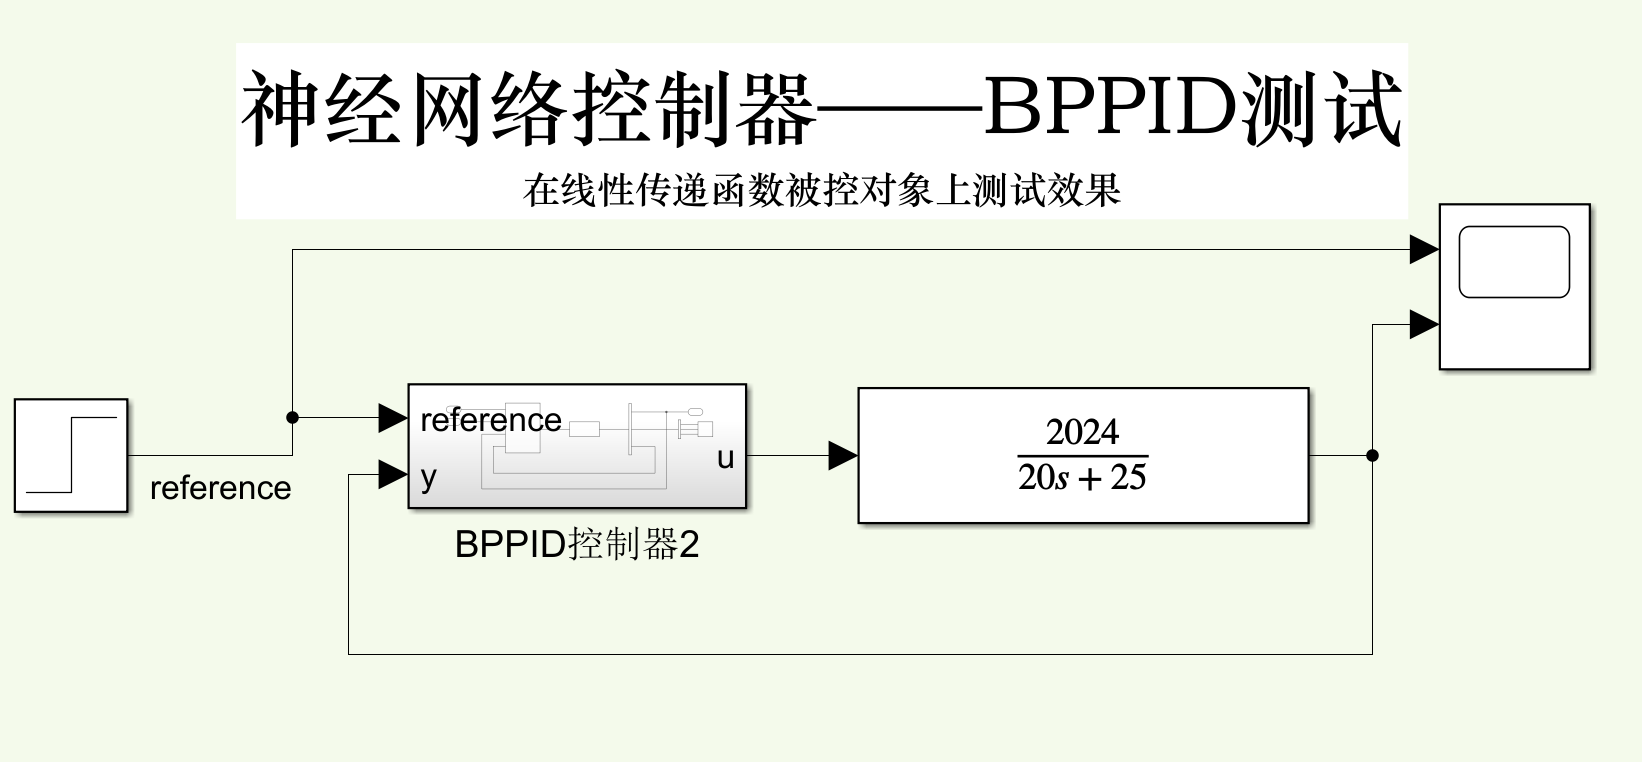
\includegraphics[width=0.4\textwidth]{2024-12-30-13-35-29.png} \caption{一阶传递函数被控对象}\end{figure}

\begin{figure}[htbp] \centering 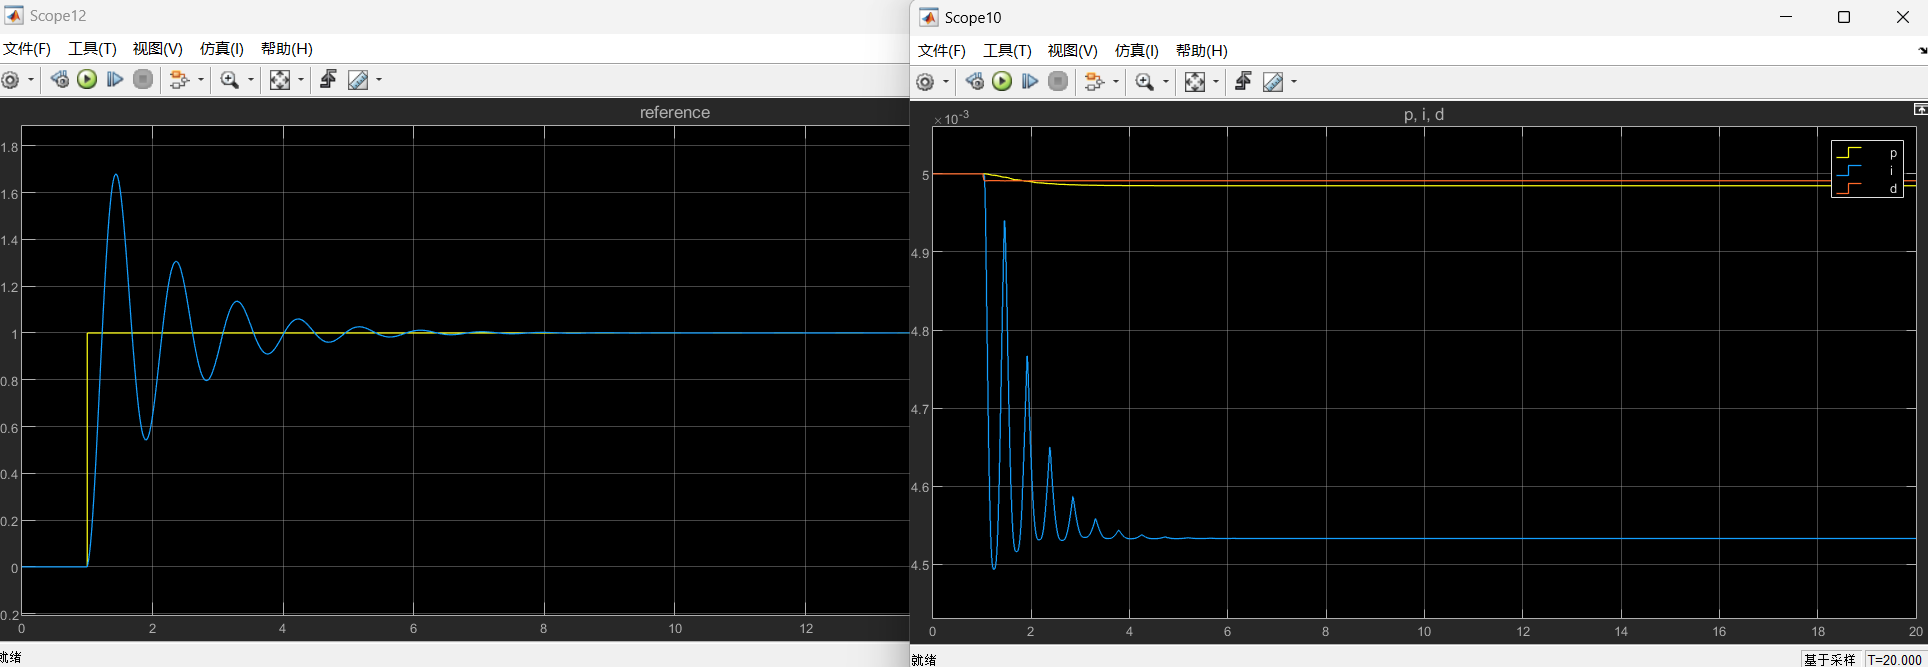
\includegraphics[width=\textwidth]{2024-12-30-13-36-45.png} \caption{一阶传递函数被控对象仿真结果}\label{fig:one_order_system}\end{figure}


\begin{figure}[htbp] \centering 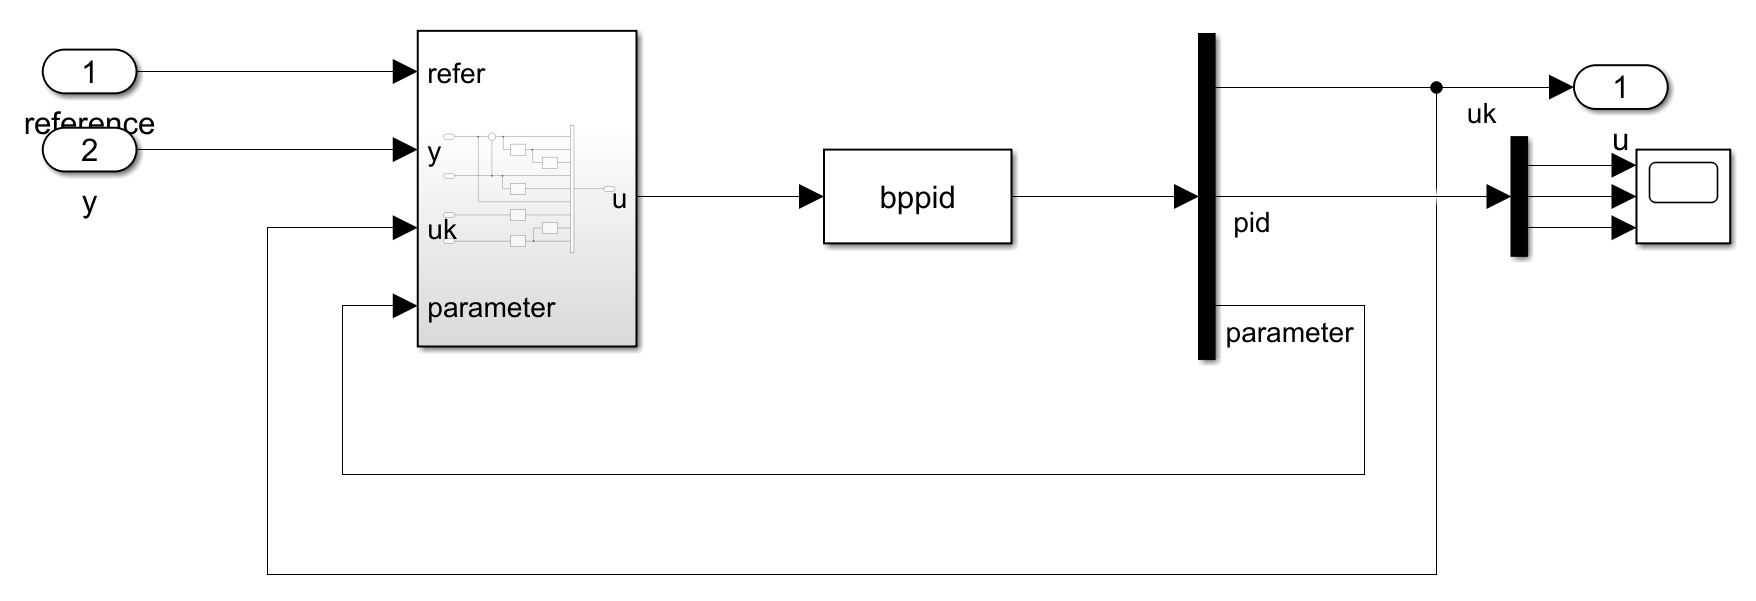
\includegraphics[width=0.7\textwidth]{2024-12-30-13-33-09.png} \caption{控制器内部结构}\end{figure}

在一阶传递函数仿真结束后,我尝试将BP-PID控制器应用到永磁同步电机的速度控制中,在经过多次调整学习率和动量因子之后,得到了以下结果。
\begin{figure}[htbp] \centering 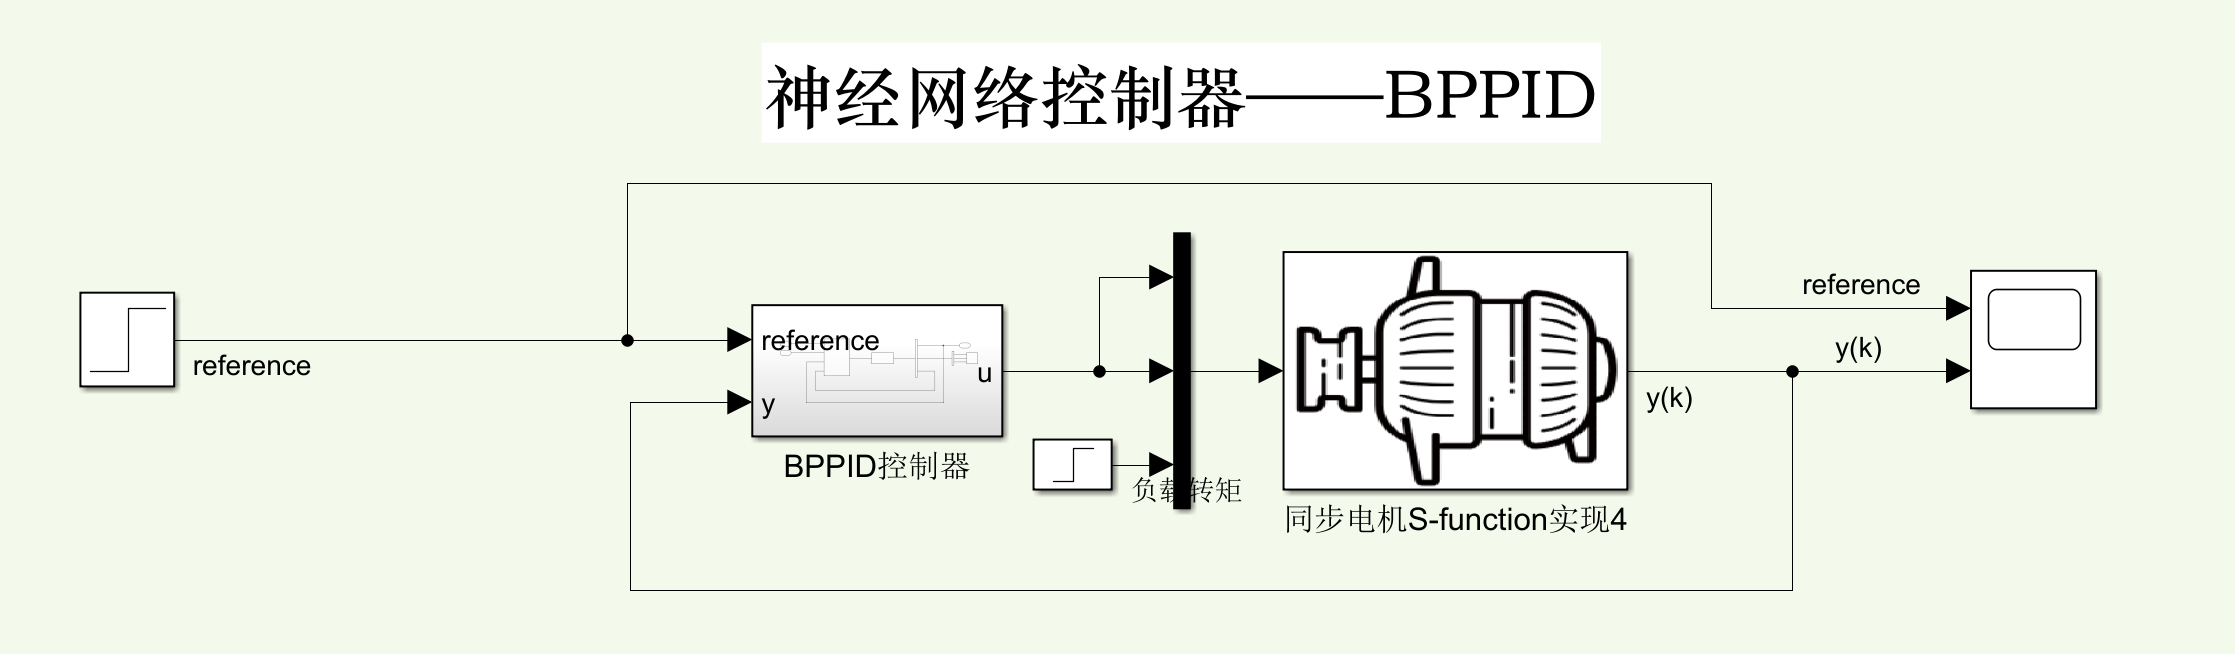
\includegraphics[width=0.7\textwidth]{2024-12-30-13-32-46.png} \caption{BP-PID控制器}\end{figure}



在PID控制器的设计过程中,要注意初始值的范围不能太离谱。因为系统不是静态的,所以初始值不能太离谱。


\begin{figure}[htbp] \centering 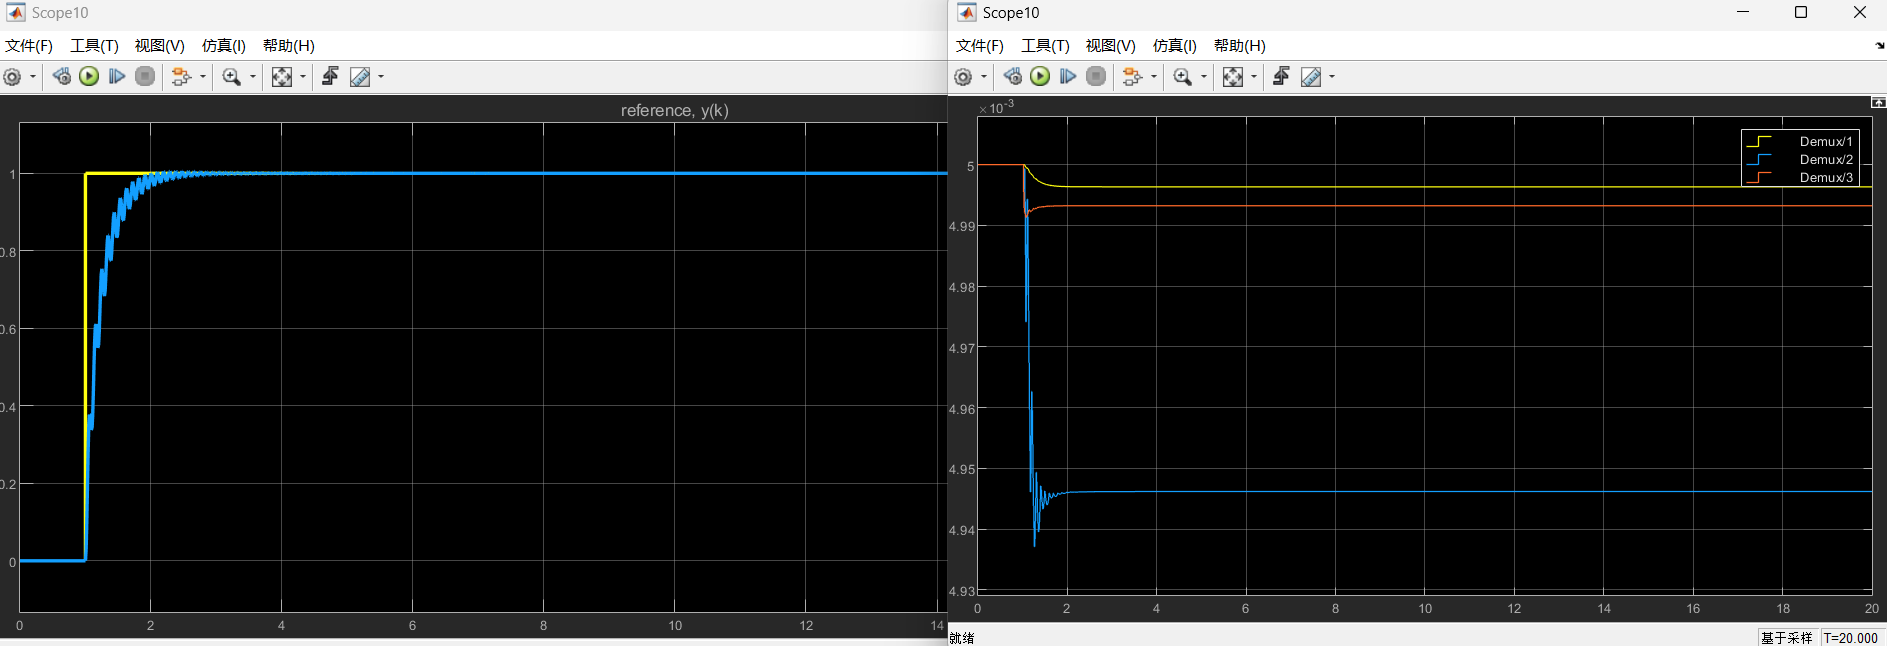
\includegraphics[width=0.7\textwidth]{2024-12-30-13-41-08.png} \caption{永磁同步电机速度控制仿真结果}\end{figure}

同时,为了加快计算速度,我尝试使用ReLU作为隐藏层的激活函数。ReLU的数学表达式为:

\begin{equation}
f(x) = \max(0,x) = \begin{cases}
x, & x > 0 \\
0, & x \leq 0
\end{cases}
\end{equation}

其导数为:
\begin{equation}
f'(x) = \begin{cases}
1, & x > 0 \\
0, & x \leq 0
\end{cases}
\end{equation}

ReLU的主要优点是:
\begin{itemize}
\item 计算简单,导数计算也很简单
\item 能缓解梯度消失问题
\item 具有稀疏性,可以让一部分神经元的输出为0
\end{itemize}

但在本实验中使用ReLU效果并不理想,所以最终没有采用这个方案。

\newpage
\subsection{RBF网络}

在BP-PID控制器之外,我还尝试使用了RBF网络来实现神经网络控制。

RBF(Radial Basis Function)网络是一种前馈神经网络,其核心思想是利用高斯核函数计算输入的非线性映射,主要用于逼近非线性函数和分类任务。更新过程的核心在于调整权值 \( w \) 和其他参数,使网络输出逐渐逼近目标值。

主要代码如下

\begin{lstlisting}[language=Matlab,caption=RBF神经网络控制器实现]
    function [sys,x0,str,ts,simStateCompliance] = rbfpid(t,x,u,flag)
    % RBF神经网络PID控制器
    % 网络结构: 3-6-1
    % 输入: 误差e、误差积分、误差微分
    % 输出: 控制量u
    
    % 采样时间
    Ts = 0.001;
    
    switch flag
        case 0
            [sys,x0,str,ts,simStateCompliance] = mdlInitializeSizes(Ts);
        case 2
            sys = mdlUpdate(x,u,Ts);
        case 3
            sys = mdlOutputs(t,x,u);
        case {1,4,9}
            sys = [];
        otherwise
            DAStudio.error('Simulink:blocks:unhandledFlag', num2str(flag));
    end
    
function [sys,x0,str,ts,simStateCompliance] = mdlInitializeSizes(Ts)
    sizes = simsizes;
    
    sizes.NumContStates  = 0;      % 连续状态个数
    sizes.NumDiscStates  = 3;      % 离散状态个数
    sizes.NumOutputs     = 5;      % 输出个数
    sizes.NumInputs      = 4;      % 输入个数
    sizes.DirFeedthrough = 1;      % 直通标志
    sizes.NumSampleTimes = 1;      % 采样时间个数
    
    sys = simsizes(sizes);
    x0  = [0;0;0];                 % 初始状态
    str = [];
    ts  = [Ts 0];                  % 采样时间
    simStateCompliance = 'UnknownSimState';
    
function sys = mdlUpdate(x,u,Ts)
    % 更新离散状态
    sys = [u(1);                   % 误差e(k)
           x(2) + u(1)*Ts;         % 误差积分
           (u(1) - u(2))];         % 误差微分e(k)-e(k-1)
    
function sys = mdlOutputs(t,x,u)
    persistent weights weights_prev weights_prev2 hidden_output centers pid_params
    
    % 学习参数设置
    learning_rate_pid = [0.01 0.01 1];    % PID参数学习率
    learning_rate_rbf = 0.06;             % RBF网络学习率
    momentum = 0.3;                       % 动量因子
    gaussian_width = 5;                   % 高斯函数宽度
    
    if t == 0
        % 初始化参数
        pid_params = [0.1 0.2 0.1];       % PID参数初值[Kp Ki Kd]
        % 初始化高斯基函数中心
        centers = [linspace(-1,1,6);      % 误差范围
                  linspace(0,1,6);        % 积分范围
                  linspace(0,1,6)];       % 微分范围
        hidden_output = zeros(6,1);       % 隐层输出
        weights = zeros(6,1);             % 网络权值
        weights_prev = weights;           % 上一次权值
        weights_prev2 = weights_prev;     % 上上次权值
    end

    % 计算PID控制器输出
    control_output = pid_params*x;
    
    % RBF网络输入
    rbf_input = [control_output u(3) u(4)]';

    % 计算隐层输出
    for j = 1:6
        hidden_output(j) = exp(-norm(rbf_input - centers(:,j))^2/(2*gaussian_width^2));
    end
    
    % 计算网络输出
    network_output = weights'*hidden_output;
    
    % 更新网络权值
    delta_weights = learning_rate_rbf*(u(3) - network_output)*hidden_output;
    weights = weights_prev + delta_weights + momentum*(weights_prev - weights_prev2);

    % 计算雅可比矩阵
    jacobian = weights.*hidden_output.*(-rbf_input(1) + centers(1,:))'/gaussian_width^2;   
    delta_output = sum(jacobian);
    
    % 更新PID参数(限制为非负)
    pid_params = max(pid_params + u(1) * delta_output * x' .* learning_rate_pid, 0);
    
    % 保存历史权值
    weights_prev2 = weights_prev;
    weights_prev = weights;
    
    % 输出结果
    sys = [control_output;network_output;pid_params(:)];
\end{lstlisting}

RBF的计算流程是这样的

1. \textbf{输入层计算}
   \begin{equation}
   \begin{aligned}
   u_{PID} &= \mathbf{K}_{PID} \cdot \mathbf{x} \\
   \mathbf{x}_{RBF} &= [u_{PID}, e(k), \dot{e}(k)]^T
   \end{aligned}
   \end{equation}
   其中$\mathbf{K}_{PID}$为PID参数向量,$\mathbf{x}$为PID控制器的输入向量。

2. \textbf{隐含层高斯激活函数计算}
   \begin{equation}
   h_j = \exp\left(-\frac{\|\mathbf{x}_{RBF} - \mathbf{c}_j\|^2}{2b^2}\right), \quad j=1,\ldots,6
   \end{equation}
   其中$\mathbf{c}_j$为第$j$个高斯基函数的中心向量,$b$为高斯函数的宽度参数。

3. \textbf{输出层计算}
   \begin{equation}
   y_{out} = \mathbf{w}^T\mathbf{h}
   \end{equation}
   其中$\mathbf{w}$为输出层权值向量,$\mathbf{h}$为隐含层输出向量。

4. \textbf{权值更新}
   \begin{equation}
   \begin{aligned}
   \Delta\mathbf{w} &= \eta(y_d - y_{out})\mathbf{h} \\
   \mathbf{w}(k) &= \mathbf{w}(k-1) + \Delta\mathbf{w} + \alpha[\mathbf{w}(k-1) - \mathbf{w}(k-2)]
   \end{aligned}
   \end{equation}
   其中$\eta$为学习率,$\alpha$为动量因子,$y_d$为期望输出。

5. \textbf{Jacobian矩阵计算}
   \begin{equation}
   \mathbf{J} = \mathbf{w} \odot \mathbf{h} \odot \frac{-\mathbf{x}_{RBF}(1) + \mathbf{c}_1}{b^2}
   \end{equation}
   其中$\odot$表示Hadamard积(逐元素相乘)。

通过以上计算流程,RBF网络可以实现对非线性系统的在线辨识和控制。其中高斯基函数提供了输入空间的局部响应特性,而权值的在线调整则保证了网络的自适应学习能力。


了解RBF网络的计算流程之后,我尝试在simulink中搭建RBF神经网络,并同样首先在一阶传递函数被控对象上进行了尝试,发现可以很好的控制。


\begin{figure}[htbp]
    \begin{minipage}{0.48\textwidth}
        \centering
        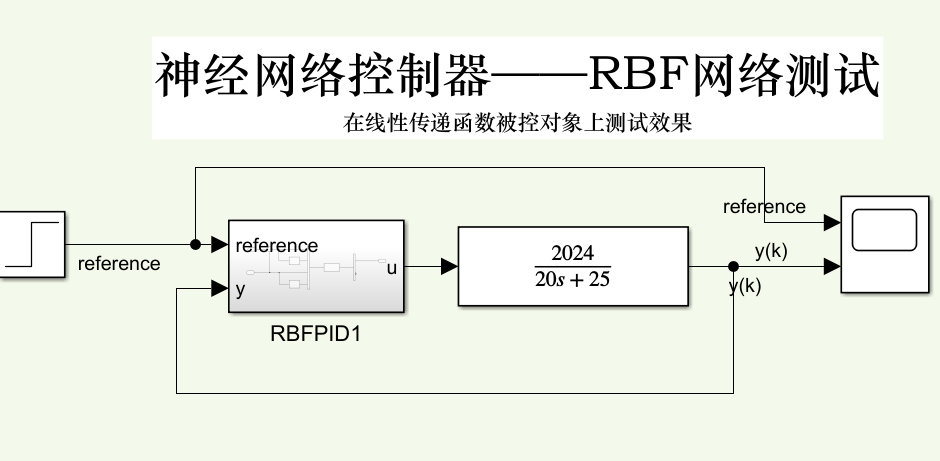
\includegraphics[width=\textwidth]{2024-12-30-14-03-28.png}
        \caption{一阶传递函数被控对象}
    \end{minipage}
    \hfill
    \begin{minipage}{0.48\textwidth}
        \centering
        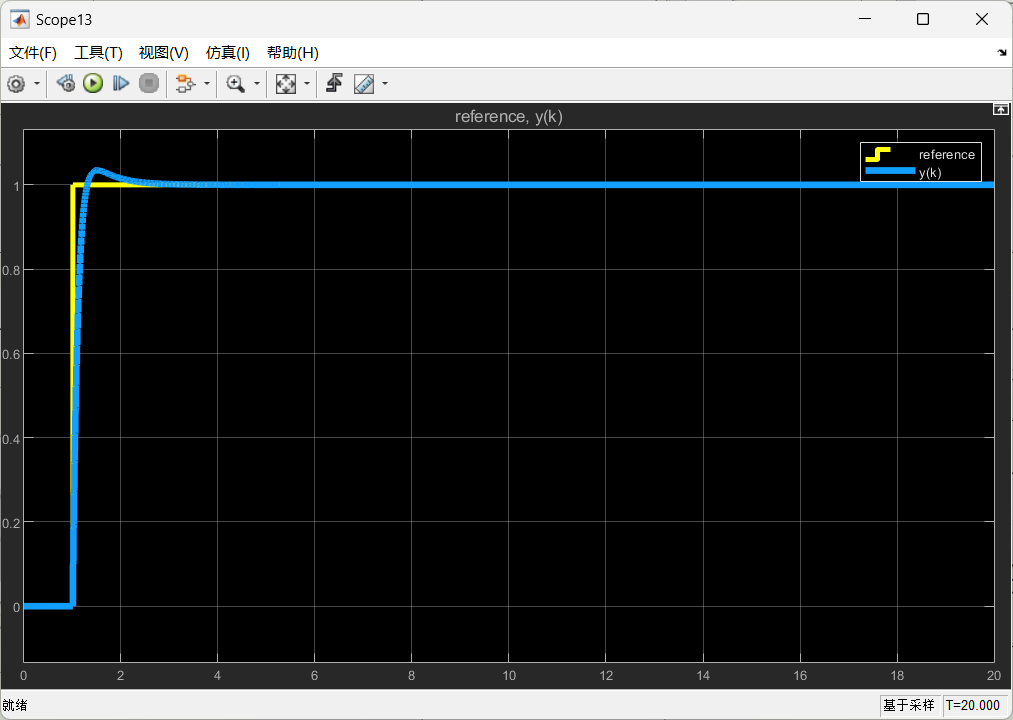
\includegraphics[width=0.9\textwidth]{2024-12-30-14-03-11.png}
        \caption{一阶传递函数被控对象仿真结果}
    \end{minipage}
\end{figure}
\newpage
在验证了RBF网络的控制效果之后,我尝试将RBF网络应用到永磁同步电机的速度控制中,结果如图\ref{fig:rbf}所示

\begin{figure}[htbp]
    \begin{minipage}{0.48\textwidth}
        \centering
        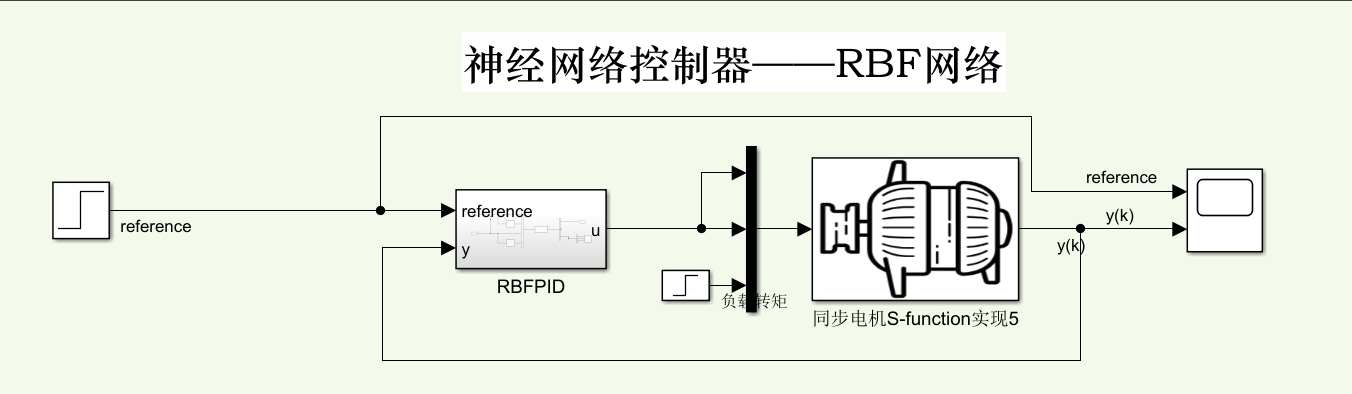
\includegraphics[width=\textwidth]{2024-12-30-13-58-24.png}
        \caption{RBF神经网络结构}\label{fig:rbf_simulink}
    \end{minipage}
    \hfill
    \begin{minipage}{0.48\textwidth}
        \centering
        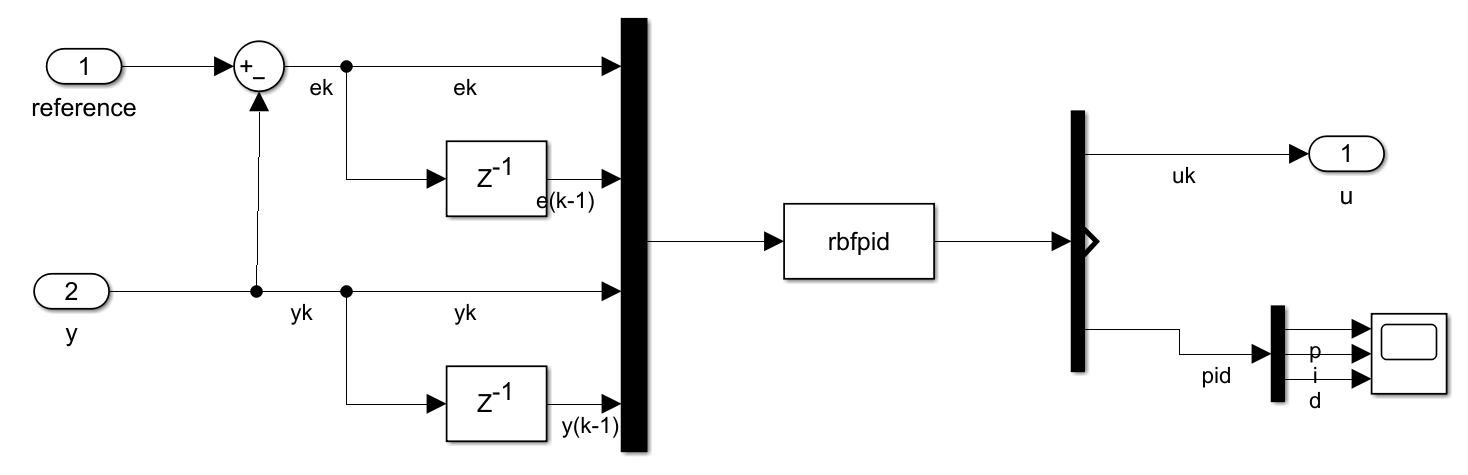
\includegraphics[width=\textwidth]{2024-12-30-14-00-16.png}
        \caption{RBF控制器内部结构}
    \end{minipage}
\end{figure}


\begin{figure}[htbp] \centering 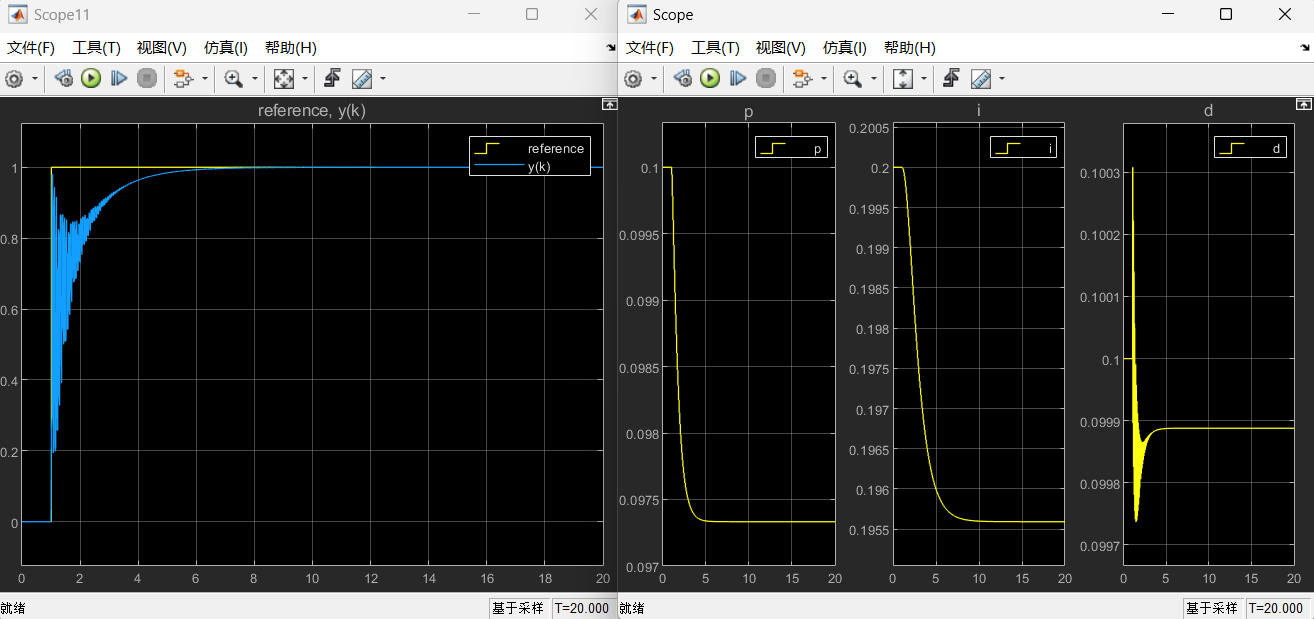
\includegraphics[width=0.7\textwidth]{2024-12-30-14-05-25.png} \caption{永磁同步电机速度控制仿真结果} \label{fig:rbf}\end{figure}

\clearpage
\section{结果比较}

在比较了各个控制器之后,我得到了如下的结果:


从仿真结果中,虽然各个控制器的表现都很好,但是可以对四种控制器的性能进行对比分析:

\begin{table}[htbp]
    \centering
    \caption{各控制器性能指标对比}
    \begin{tabular}{|c|c|c|c|}
        \hline
        控制器类型 & 稳定时间 & 超调量 & 稳态误差 \\
        \hline
        模糊PID控制器 & 最短 & 较大 & 最小 \\
        \hline
        BPPID控制器 & 较短 & 最小 & 最小 \\
        \hline
        RBF神经网络控制器 & 较慢 & 较小 & 较小 \\
        \hline
        模糊控制器 & 较慢 & 较大 & 较大 \\
        \hline
    \end{tabular}
    \label{tab:controller_comparison}
\end{table}

从表\ref{tab:controller_comparison}中可以看出:

\begin{itemize}
    \item \textbf{稳定时间}方面:模糊PID控制器表现最好,达到稳态时间最短;其次是BPPID控制器;RBF和模糊控制器相对较慢。
    
    \item \textbf{超调量}方面:BPPID神经网络控制器的超调最小;RBF次之;而模糊PID和模糊控制器的超调量相对较大。
    
    \item \textbf{稳态误差}方面:模糊PID和BPPID控制器的稳态误差最小;RBF神经网络控制器次之;模糊控制器的稳态误差相对较大。
\end{itemize}



\clearpage
\section{Matlab工具包学习记录}

\subsection{Deep Learning Toolbox 学习}

首先我根据助教的视频,和b站上的视频,学习了神经网络工具箱的基本用法,具体用到的数据和代码放到\texttt{learn\_toolbox}文件夹中

当然,使用工具箱自带的一些数据集也是可以的。

\begin{lstlisting}[language=Matlab,caption=打开神经网络工具箱]
nftool
\end{lstlisting}

\begin{itemize}
    \item 选择导入数据集
    \item 正确选择是行还是列
    \item 选择训练集的比例;隐藏层的个数(5or10)
    \item 选择训练方法:一般选择第一个方法;第二个方法和遗传算法一起用;第三个方法比较慢
\end{itemize}

\textbf{提示:} validation test 表示的是泛化性能,如果连续6个epoch都上不去,就停止训练

图像查看:一般看回归的图(第四个),如果都上了0.9差不多就可以了

\textbf{模型保存}

\begin{lstlisting}[language=Matlab,caption=保存模型]
save('filename.mat')  % 保存所有变量
save('filename.mat', 'var1', 'var2')  % 只保存指定变量
\end{lstlisting}

\begin{lstlisting}[language=Matlab,caption=从.mat文件中导入数据]
load('data.mat');
\end{lstlisting}

\textbf{模型预测}

\begin{lstlisting}[language=Matlab,caption=方法1:使用sim函数]
PreY = zeros(10,1);
for i = 1:10
    PreY(i,1) = sim(net,PreX(i,:)');
    % sim函数第二个参数列数等于输入向量的个数
end
disp(PreY);
\end{lstlisting}

\begin{lstlisting}[language=Matlab,caption=方法2:使用生成的函数]
myNeuralNetworkFunction(X) % 这里需要把后两个参数去掉
\end{lstlisting}
 
\textbf{多输入多输出}

多输入多输出也是一样的操作,唯一值得注意的地方就是在训练之前需要将行还是列选择正确(特征or样本)

\textbf{使用脚本替代ui操作}

\begin{lstlisting}[language=Matlab,caption=使用脚本替代ui操作,并且函数化]
function train()
    dataFile = 'data.mat';
    load(dataFile);  % 从文件导入数据
    x = features';  % 转置为符合网络输入格式
    t = labels';  % 转置为符合网络目标格式

    % 选择训练函数
    trainFcn = 'trainlm';  % Levenberg-Marquardt 反向传播

    % 创建拟合网络
    hiddenLayerSize = 15;
    net = fitnet(hiddenLayerSize, trainFcn);

    % 输入输出的预处理函数
    net.input.processFcns = {'removeconstantrows', 'mapminmax'};
    net.output.processFcns = {'removeconstantrows', 'mapminmax'};

    % 设置数据的划分方式
    net.divideFcn = 'dividerand';  % 随机划分数据
    net.divideMode = 'sample';  % 划分所有样本
    net.divideParam.trainRatio = 70/100;
    net.divideParam.valRatio = 15/100;
    net.divideParam.testRatio = 15/100;

    % 选择性能函数
    net.performFcn = 'mse';  % 均方误差

    % 选择绘图函数
    net.plotFcns = {'plotperform', 'plottrainstate', 'ploterrhist', ...
        'plotregression', 'plotfit'};

    % 训练网络
    [net, tr] = train(net, x, t);

    % 测试网络
    y = net(x);
    e = gsubtract(t, y);
    performance = perform(net, t, y);

    % 重新计算训练、验证和测试性能
    trainTargets = t .* tr.trainMask{1};
    valTargets = t .* tr.valMask{1};
    testTargets = t .* tr.testMask{1};
    trainPerformance = perform(net, trainTargets, y);
    valPerformance = perform(net, valTargets, y);
    testPerformance = perform(net, testTargets, y);

    figure, plotperform(tr);% 绘制并保存训练性能图
%     figure, plottrainstate(tr);% 绘制并保存训练状态图
%     figure, ploterrhist(e);% 绘制并保存误差直方图
    figure, plotregression(t, y)
%     figure, plotfit(net, x, t);% 绘制并保存拟合图

    % 保存模型
%     modelFile = ['model_level' num2str(level) '.mat'];
%     save(modelFile, 'net');  % 保存神经网络模型
    % 生成simulink模型
    gensim(net);
    disp(['Model saved as ' modelFile]);
end
\end{lstlisting}

使用Control System Designer进行自动调参,可以大大提高调参效率。

\begin{figure}[htbp] \centering 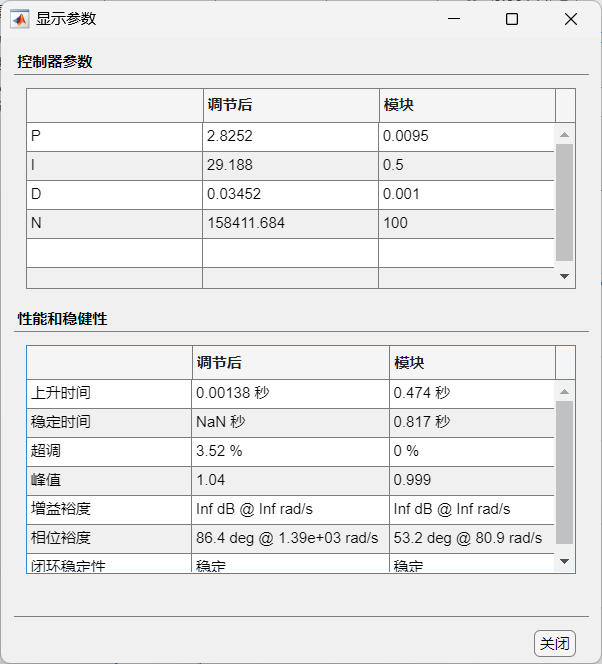
\includegraphics[width=0.3\textwidth]{2024-12-30-11-56-41.png} \caption{Control System Designer自动调参}\end{figure}

界面如下,拖动两个按钮可以修改曲线参数,按下按钮两边得大于/小于号,可以拓宽,收缩调节范围。
\begin{figure}[htbp] \centering 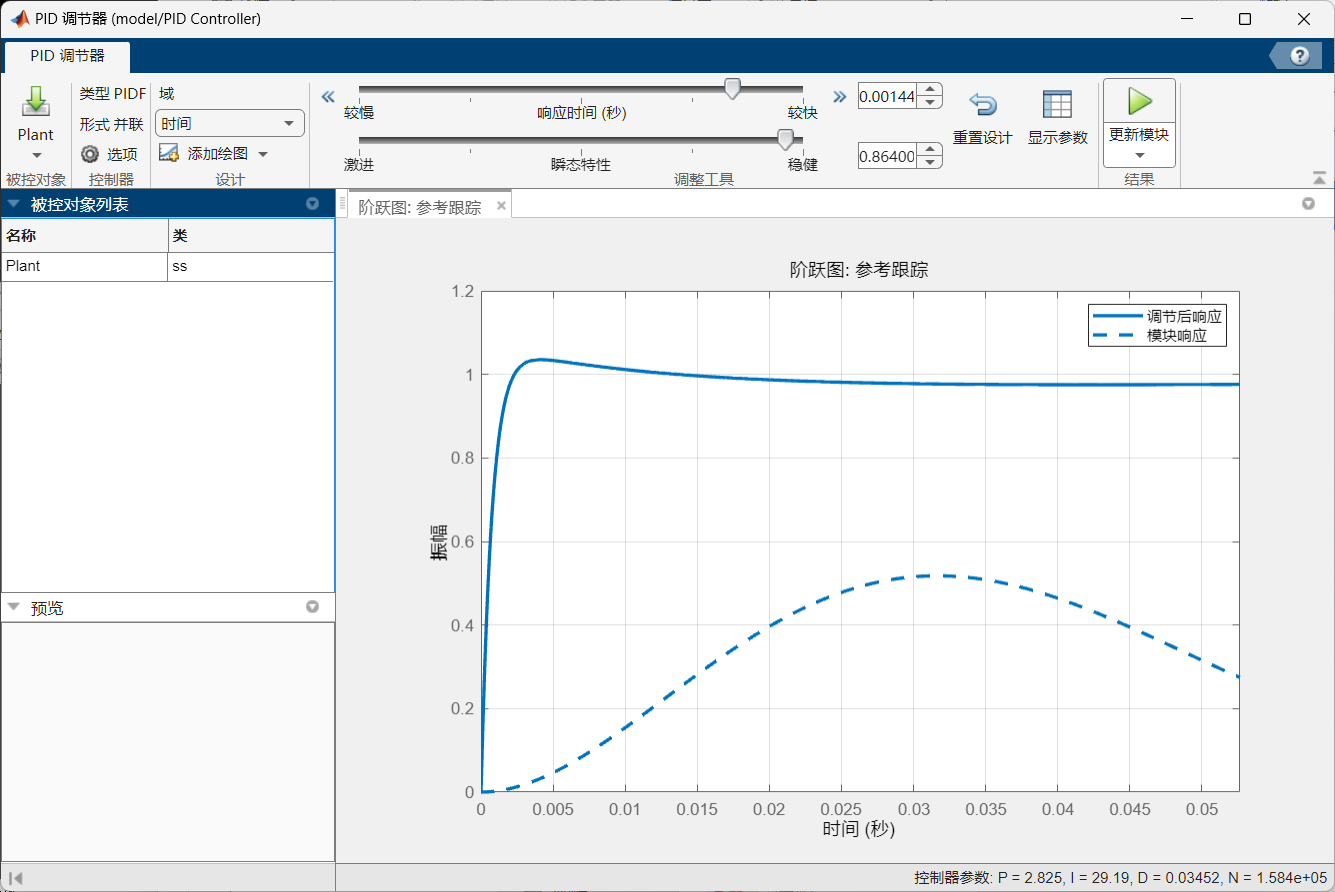
\includegraphics[width=0.4\textwidth]{2024-12-30-11-56-53.png} \caption{Control System Designer自动调参结果}\end{figure}


点击show Parameter 显示曲线信息,有曲线的超调量,增益,达到设定值的时间,曲线是否稳定等。可以边拖动曲线,边看表格。

可以看到有两条曲线,一条是上次PID值下得曲线,一条是目前PID值下得曲线。

找到比较合适的曲线,更新到simulink中,点击update 按钮,就可以更新到simulink中。

\subsection{MPC Designer学习}



\clearpage
\appendix


\section{附录1:文件夹结构}
\begin{figure}[htbp] \centering 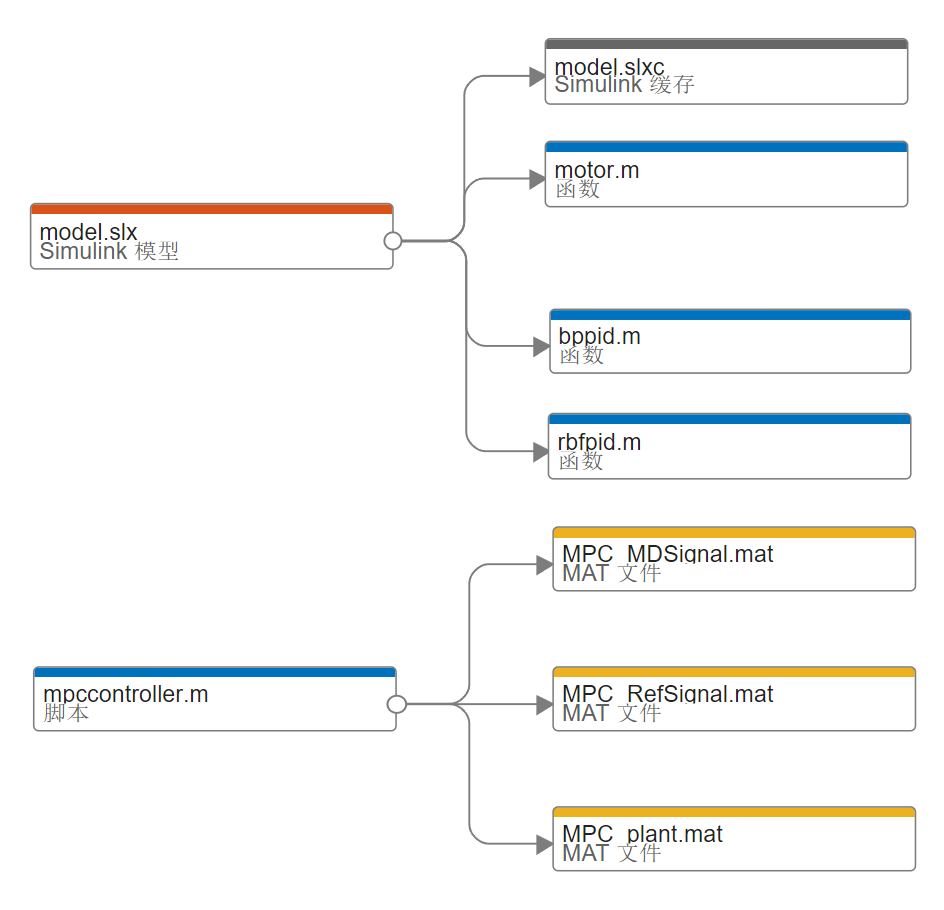
\includegraphics[width=0.4\textwidth]{依存关系图.png} \caption{文件依存关系图}\end{figure}

\dirtree{%
.1 .
.2 README.md\DTcomment{项目说明文件}.
.2 assets\DTcomment{存放图片资源的文件夹}.
.2 report.
.3 thesis.tex\DTcomment{主要的LaTeX源文件}.
.3 thesis.pdf\DTcomment{生成的PDF报告}.
.2 src\DTcomment{源代码文件夹}.
.3 bppid.m\DTcomment{BP神经网络PID控制器实现}.
.3 Fuzzy\_Control.fis\DTcomment{模糊控制器设计文件}.
.3 Fuzzy\_PID.fis\DTcomment{模糊PID控制器设计文件}.
.3 model.slx\DTcomment{Simulink模型文件}.
.3 model.slxc\DTcomment{Simulink缓存文件}.
.3 motor.m\DTcomment{电机模型实现}.
.3 mpccontroller.m\DTcomment{MPC控制器实现}.
.3 Project.prj\DTcomment{项目配置文件}.
.3 rbfpid.m\DTcomment{RBF神经网络PID控制器实现}.
.3 test.fis\DTcomment{测试用模糊系统文件}.
.2 thesis\DTcomment{参考文献文件夹}.
.3 一种永磁同步电机无模型高阶滑模控制算法\_赵凯辉.pdf\DTcomment{参考论文}.
.3 空间矢量坐标变换(等幅值变换) - 知乎.html\DTcomment{参考资料}.
.3 空间矢量坐标变换(等幅值变换) - 知乎\_files\DTcomment{参考资料附件}.
}

\newpage
\section{附录2:版本更新记录}


\begin{table}[htbp]
\centering
\caption{版本更新记录}
\begin{tabular}{|c|l|}
\hline
时间 & 更新内容 \\
\hline
12.27上午 & 完成PID控制器设计与调参 \\
\hline
12.27下午 & 完成Control System Designer自动调参与实验 \\
\hline
12.28上午 & 完成MPC模型预测控制器设计与实现 \\
\hline
12.29上午 & 完成模糊控制器设计与模糊PID控制实现 \\
\hline
12.30上午 & 完成BP-PID神经网络控制器设计 \\
\hline
12.30下午 & 完成RBF神经网络控制器实现与测试 \\
\hline
12.31下午 & 完成实验结果分析与报告撰写 \\
\hline
\end{tabular}
\end{table}

\reference

\clearpage
\section{附录3:总结与经验感悟}

通过半个学期的学习,我从一个完全不会使用simulink的小白,现在可以在simulink中快速搭建一个模型进行仿真的实验。非常感谢老师和助教的指导。

智能控制这门课程算是比较硬核的,4个小作业,每个作业都涉及到了不同的控制方法,并且需要使用不同的工具箱,而大作业则是需要将这些方法结合起来,完成一个控制的系统的搭建。学习各个工具包的用法确实是需要很多时间和精力投入的,每次作业我都要花蛮久的时间进行学习和实验,但是我觉得投入的时间确实学到了很多东西。学到的专家控制和模糊控制方法也用在了另一门课程的大作业课程设计中。

比较痛苦的是作业可能缺少一些难度的阶梯,比如在每次小作业讲解的时候,如果可以安排一个小例子或者简单的模型来验证工具包安装和使用的正确性,那么可能可以减少很多同学的疑惑。

在本门课程中,我也整理了一些我在课堂的笔记和实验上的一些心得,放在了我的个人网站上,可以访问下边的链接查看\href{https://www.philfan.cn/Robotics/Control/Control-11-%E6%99%BA%E8%83%BD%E6%8E%A7%E5%88%B6%E6%96%B9%E6%B3%95/}{课程笔记},\href{https://www.philfan.cn/Tools/matlab/}{matlab工具包学习记录}
\end{document}
